% Options for packages loaded elsewhere
\PassOptionsToPackage{unicode}{hyperref}
\PassOptionsToPackage{hyphens}{url}
%
\documentclass[
]{article}
\usepackage{lmodern}
\usepackage{amsmath}
\usepackage{ifxetex,ifluatex}
\ifnum 0\ifxetex 1\fi\ifluatex 1\fi=0 % if pdftex
  \usepackage[T1]{fontenc}
  \usepackage[utf8]{inputenc}
  \usepackage{textcomp} % provide euro and other symbols
  \usepackage{amssymb}
\else % if luatex or xetex
  \usepackage{unicode-math}
  \defaultfontfeatures{Scale=MatchLowercase}
  \defaultfontfeatures[\rmfamily]{Ligatures=TeX,Scale=1}
\fi
% Use upquote if available, for straight quotes in verbatim environments
\IfFileExists{upquote.sty}{\usepackage{upquote}}{}
\IfFileExists{microtype.sty}{% use microtype if available
  \usepackage[]{microtype}
  \UseMicrotypeSet[protrusion]{basicmath} % disable protrusion for tt fonts
}{}
\makeatletter
\@ifundefined{KOMAClassName}{% if non-KOMA class
  \IfFileExists{parskip.sty}{%
    \usepackage{parskip}
  }{% else
    \setlength{\parindent}{0pt}
    \setlength{\parskip}{6pt plus 2pt minus 1pt}}
}{% if KOMA class
  \KOMAoptions{parskip=half}}
\makeatother
\usepackage{xcolor}
\IfFileExists{xurl.sty}{\usepackage{xurl}}{} % add URL line breaks if available
\IfFileExists{bookmark.sty}{\usepackage{bookmark}}{\usepackage{hyperref}}
\hypersetup{
  pdftitle={Molecular Ecology Chaps 0-3 UnShiny},
  pdfauthor={John Wares},
  hidelinks,
  pdfcreator={LaTeX via pandoc}}
\urlstyle{same} % disable monospaced font for URLs
\usepackage[margin=1in]{geometry}
\usepackage{color}
\usepackage{fancyvrb}
\newcommand{\VerbBar}{|}
\newcommand{\VERB}{\Verb[commandchars=\\\{\}]}
\DefineVerbatimEnvironment{Highlighting}{Verbatim}{commandchars=\\\{\}}
% Add ',fontsize=\small' for more characters per line
\usepackage{framed}
\definecolor{shadecolor}{RGB}{248,248,248}
\newenvironment{Shaded}{\begin{snugshade}}{\end{snugshade}}
\newcommand{\AlertTok}[1]{\textcolor[rgb]{0.94,0.16,0.16}{#1}}
\newcommand{\AnnotationTok}[1]{\textcolor[rgb]{0.56,0.35,0.01}{\textbf{\textit{#1}}}}
\newcommand{\AttributeTok}[1]{\textcolor[rgb]{0.77,0.63,0.00}{#1}}
\newcommand{\BaseNTok}[1]{\textcolor[rgb]{0.00,0.00,0.81}{#1}}
\newcommand{\BuiltInTok}[1]{#1}
\newcommand{\CharTok}[1]{\textcolor[rgb]{0.31,0.60,0.02}{#1}}
\newcommand{\CommentTok}[1]{\textcolor[rgb]{0.56,0.35,0.01}{\textit{#1}}}
\newcommand{\CommentVarTok}[1]{\textcolor[rgb]{0.56,0.35,0.01}{\textbf{\textit{#1}}}}
\newcommand{\ConstantTok}[1]{\textcolor[rgb]{0.00,0.00,0.00}{#1}}
\newcommand{\ControlFlowTok}[1]{\textcolor[rgb]{0.13,0.29,0.53}{\textbf{#1}}}
\newcommand{\DataTypeTok}[1]{\textcolor[rgb]{0.13,0.29,0.53}{#1}}
\newcommand{\DecValTok}[1]{\textcolor[rgb]{0.00,0.00,0.81}{#1}}
\newcommand{\DocumentationTok}[1]{\textcolor[rgb]{0.56,0.35,0.01}{\textbf{\textit{#1}}}}
\newcommand{\ErrorTok}[1]{\textcolor[rgb]{0.64,0.00,0.00}{\textbf{#1}}}
\newcommand{\ExtensionTok}[1]{#1}
\newcommand{\FloatTok}[1]{\textcolor[rgb]{0.00,0.00,0.81}{#1}}
\newcommand{\FunctionTok}[1]{\textcolor[rgb]{0.00,0.00,0.00}{#1}}
\newcommand{\ImportTok}[1]{#1}
\newcommand{\InformationTok}[1]{\textcolor[rgb]{0.56,0.35,0.01}{\textbf{\textit{#1}}}}
\newcommand{\KeywordTok}[1]{\textcolor[rgb]{0.13,0.29,0.53}{\textbf{#1}}}
\newcommand{\NormalTok}[1]{#1}
\newcommand{\OperatorTok}[1]{\textcolor[rgb]{0.81,0.36,0.00}{\textbf{#1}}}
\newcommand{\OtherTok}[1]{\textcolor[rgb]{0.56,0.35,0.01}{#1}}
\newcommand{\PreprocessorTok}[1]{\textcolor[rgb]{0.56,0.35,0.01}{\textit{#1}}}
\newcommand{\RegionMarkerTok}[1]{#1}
\newcommand{\SpecialCharTok}[1]{\textcolor[rgb]{0.00,0.00,0.00}{#1}}
\newcommand{\SpecialStringTok}[1]{\textcolor[rgb]{0.31,0.60,0.02}{#1}}
\newcommand{\StringTok}[1]{\textcolor[rgb]{0.31,0.60,0.02}{#1}}
\newcommand{\VariableTok}[1]{\textcolor[rgb]{0.00,0.00,0.00}{#1}}
\newcommand{\VerbatimStringTok}[1]{\textcolor[rgb]{0.31,0.60,0.02}{#1}}
\newcommand{\WarningTok}[1]{\textcolor[rgb]{0.56,0.35,0.01}{\textbf{\textit{#1}}}}
\usepackage{graphicx}
\makeatletter
\def\maxwidth{\ifdim\Gin@nat@width>\linewidth\linewidth\else\Gin@nat@width\fi}
\def\maxheight{\ifdim\Gin@nat@height>\textheight\textheight\else\Gin@nat@height\fi}
\makeatother
% Scale images if necessary, so that they will not overflow the page
% margins by default, and it is still possible to overwrite the defaults
% using explicit options in \includegraphics[width, height, ...]{}
\setkeys{Gin}{width=\maxwidth,height=\maxheight,keepaspectratio}
% Set default figure placement to htbp
\makeatletter
\def\fps@figure{htbp}
\makeatother
\setlength{\emergencystretch}{3em} % prevent overfull lines
\providecommand{\tightlist}{%
  \setlength{\itemsep}{0pt}\setlength{\parskip}{0pt}}
\setcounter{secnumdepth}{-\maxdimen} % remove section numbering
\ifluatex
  \usepackage{selnolig}  % disable illegal ligatures
\fi

\title{Molecular Ecology Chaps 0-3 UnShiny}
\author{John Wares}
\date{5/26/2021}

\begin{document}
\maketitle

\hypertarget{what-is-this}{%
\section{0. What is this?}\label{what-is-this}}

Written by \textbf{J.P. Wares}, Professor, University of Georgia,
jpwares {[}at{]} uga.edu

This is shared \emph{by-nc-sa/4.0}, I'm not writing it to be some
polished final thing but something that shifts through new ideas and new
people using or modifying parts of it. This text may be used following
these guidelines:
\url{https://creativecommons.org/licenses/by-nc-sa/4.0/}

This document is being developed for the cross-listed ECOL/GENE
4530/6530 at University of Georgia to improve the experiential nature of
learning the methods necessary for the field of ``\emph{molecular
ecology}''. Maintaining it as an .Rmd allows direct analytical
opportunities (and familiarity with basic statistical coding approaches)
and the ability to incorporate some simple simulation tools using Shiny.
It will also let me update as needed in a straightforward way.

\hypertarget{why-write-this}{%
\subsection{0.1 Why write this?}\label{why-write-this}}

\hypertarget{for-most-of-my-career-as-a-biologist-ive-found-myself-wanting-to-know-why-things-are-where-they-are.-that-means-i-need-to-know-what-they-are-and-how-they-can-move-rules-like-chess-but-far-more-complex-and-varied-and-sometimes-involving-low-probabilities.-i-need-to-know-these-things-with-varying-degrees-of-precision-given-the-questions-being-asked-about-those-organisms.-the-molecular-ecology-approaches-we-will-learn-and-evaluate-in-here-have-helped-a-lot-with-this-pursuit-but-of-course-it-all-roots-in-knowing-as-much-as-you-can-about-the-organisms---life-history-ecology-development-and-maturation---otherwise.}{%
\subsubsection{\texorpdfstring{For most of my career as a biologist,
I've found myself wanting to know \emph{why things are where they are}.
That means I need to know \textbf{what} they are, and how they can move;
rules like chess but far more complex and varied, and sometimes
involving low probabilities. I need to know these things with varying
degrees of precision given the questions being asked about those
organisms. The `molecular ecology' approaches we will learn and evaluate
in here have helped a lot with this pursuit, but of course it all roots
in knowing as much as you can about the organisms - life history,
ecology, development and maturation -
otherwise.}{For most of my career as a biologist, I've found myself wanting to know why things are where they are. That means I need to know what they are, and how they can move; rules like chess but far more complex and varied, and sometimes involving low probabilities. I need to know these things with varying degrees of precision given the questions being asked about those organisms. The `molecular ecology' approaches we will learn and evaluate in here have helped a lot with this pursuit, but of course it all roots in knowing as much as you can about the organisms - life history, ecology, development and maturation - otherwise.}}\label{for-most-of-my-career-as-a-biologist-ive-found-myself-wanting-to-know-why-things-are-where-they-are.-that-means-i-need-to-know-what-they-are-and-how-they-can-move-rules-like-chess-but-far-more-complex-and-varied-and-sometimes-involving-low-probabilities.-i-need-to-know-these-things-with-varying-degrees-of-precision-given-the-questions-being-asked-about-those-organisms.-the-molecular-ecology-approaches-we-will-learn-and-evaluate-in-here-have-helped-a-lot-with-this-pursuit-but-of-course-it-all-roots-in-knowing-as-much-as-you-can-about-the-organisms---life-history-ecology-development-and-maturation---otherwise.}}

\begin{figure}

{\centering 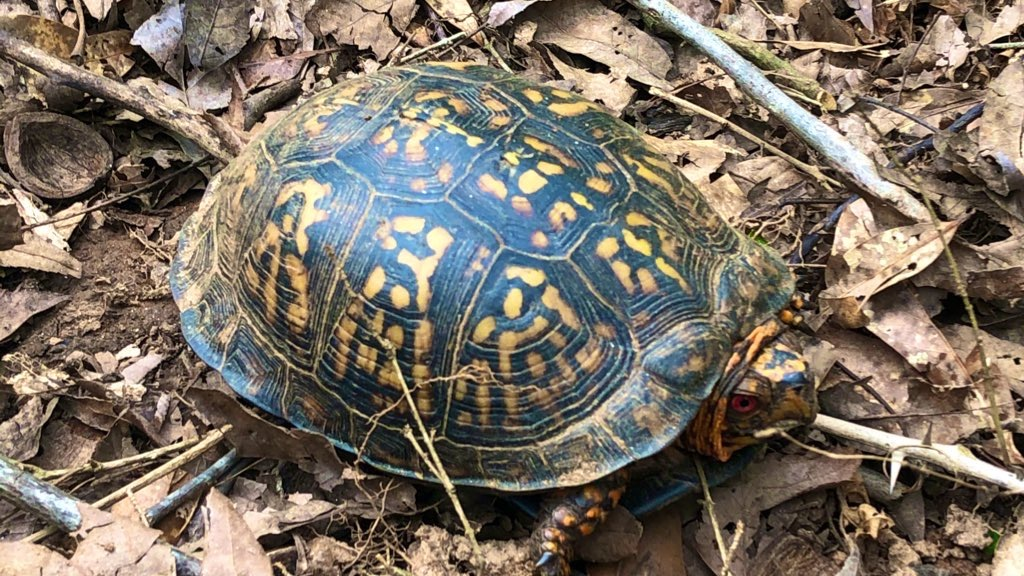
\includegraphics[width=0.9\linewidth]{MEImages/IMG_1549} 

}

\caption{...}\label{fig:unnamed-chunk-1}
\end{figure}

\textbf{Surely you already have some thoughts on how turtles move, and
what that could mean for the spatial distribution of diverse phenotypes
and molecular diversity within their range? (photo: J. Wares)}

\hypertarget{why-would-i-use-this}{%
\subsection{0.2 Why would I use this?}\label{why-would-i-use-this}}

I \emph{think}\ldots{} I think\ldots{} I'm writing this in a way that
more advanced students can skim the first few chapters and gain
something from focusing on the latter ones; a more novice course might
only get through the first several chapters and then just read
appropriate-focused papers (e.g.~in the undergrad/grad mix I expect to
teach, the course will move at one pace but the grads at another and
with a distinct type of guidance, starting to use more time later in
semester to present on methods or case studies). I want to think about
how to \emph{teach} molecular ecology, not just about how to do it. It
seems there has to be some coding expertise that comes into play at this
point, and some experiential practice. So, I think this is what is going
to work. I hope.

\hypertarget{introduction}{%
\section{1. Introduction}\label{introduction}}

The first day of classes we will prep our computers for using R/RStudio
for a major resource in this class. If at all possible, before the class
begins you should install R:

\url{https://www.r-project.org}

and RStudio (free version):

\url{https://rstudio.com/products/rstudio/}

Please note the risk in all of this is that \emph{packages} and
\emph{versions} of software are constantly changing, and sometimes code
that has been working will stop (and vice-versa) because of these
changes. Additionally, a key element of making this work - currently -
is making sure that the \emph{path} is set correctly so that this .Rmd
file can find figures and code to interact with. I'm hoping I've set
this up so that everything works from the directory you downloaded, but
we will double-check today.

\hypertarget{r-markdown-and-shiny}{%
\subsection{1.0 R Markdown and Shiny}\label{r-markdown-and-shiny}}

This is an R Markdown document, with Shiny apps built in. At this point
in time, the Shiny apps are all written by the talented Dr.~Silas Tittes
and are available at \url{https://github.com/silastittes/shiny_popgen}.

What does that mean? Markdown is a simple formatting syntax for
authoring HTML, PDF, and Microsoft Word documents. For more details on
using R Markdown see \url{http://rmarkdown.rstudio.com}. Adding the
Shiny apps means that the document is \emph{interactive}. The only
downside is that it means that users must have \textbf{R} and
\textbf{RStudio} installed, plus a few R packages, on their computer.

(OK, another downside is it is going to be difficult to read in a
hammock. Or, at least, you should read something else if you are in a
hammock.)

The upside is that it is more of a living document. It means that as
data change, the output of analysis can change. It also means that R
code can be built directly into the document so that you can see how
some figures or modules are generated, and you can build on this
knowledge. You can embed an R ``code chunk'' like this:

\begin{Shaded}
\begin{Highlighting}[]
\FunctionTok{library}\NormalTok{(learnPopGen)}
\NormalTok{driftplot}\OtherTok{\textless{}{-}}\FunctionTok{drift.selection}\NormalTok{(}\AttributeTok{p0=}\FloatTok{0.25}\NormalTok{,}\AttributeTok{Ne=}\DecValTok{500}\NormalTok{,}\AttributeTok{w=}\FunctionTok{c}\NormalTok{(}\DecValTok{1}\NormalTok{,}\DecValTok{1}\NormalTok{,}\DecValTok{1}\NormalTok{),}\AttributeTok{ngen=}\DecValTok{400}\NormalTok{,}\AttributeTok{nrep=}\DecValTok{5}\NormalTok{)}
\end{Highlighting}
\end{Shaded}

\includegraphics{ASU_MolEcol_UNshiny_files/figure-latex/driftsim-1.pdf}

I'm putting this text together using R Markdown in particular so that
examples can be incorporated that students can then work with to try and
understand how varying the input information affects our expectations
about the molecular data used to answer ecological questions. For
example, the code chunk above - and the figure it produces - not only
illustrates \emph{genetic drift} (here, an example where one of 2
alleles is initiated in a population at a frequency of 0.25, and the
``effective population size'' about which we will learn more, is 500;
there are 5 replicate simulations - in fact you should notice that the
figure is distinct every time you run this document!), but actually
provides the code for the illustration that can be modified as knowledge
of the process becomes more advanced (when looking at the R Markdown
code document itself in \emph{RStudio}, if you hit the green `play'
button in the upper right corner of the ``code chunk'' you can do the
simulation over and over, and you can look at the code and probably
figure out quickly how to change the parameters it runs under).

By organizing this material the way I think it may come across to
beginning students in the field, I hope to avoid the personal puzzle of
when I initially shifted this class from 8000-level (intermediate grad
course) to 4000-level (advanced undergrads with fewer prerequisites) by
clarifying these probabilistic processes with illustrations based on
simulations that the students can themselves repeat.

Because I'm using \textbf{Shiny} code, you cannot ``Knit'' this document
into a static form, but instead will hit ``Run Document'' (up near the
top of the RStudio screen) once it is loaded into R and that will
generate a browser text that is dynamic in some places to let \emph{you}
run the simulations. It is a work in progress, but for now it does mean
that to work with this you must have access to a computer that will run
R and RStudio, at a minimum.

This will be less a textbook that you read for complete comprehension,
and more something you read to generate questions that we discuss; I am
trying to ``flip the classroom'' and organize for future classes at the
same time. Some aspects will need to be explained in class or using
diverse media to make sense. When I was a sophomore learning cell
biology, I know that I tested well on the subject but in the end, had
zero clue what gel electrophoresis meant until I did it on a daily
basis. (super basic intro to ``electrophoresis'':
\url{https://www.youtube.com/watch?v=ZDZUAleWX78}) So, \textbf{your job
is to ask questions!} That way, we learn more completely not just from
me, but from each other and from our inquiry.

For other users of this document, please note: I use a lot of examples I
am familiar with, meaning they are often projects I'm an author on, or
was on that person's committee, or whatever. There is so much other
\emph{fantastic} science out there, this isn't about ego though: it's
just my ability to immediately dig deeper with those as examples not
just of how the science \emph{can} be done, but also about when it
\emph{could have been done better}. Also, I'm a marine ecologist; when I
talk about plants, it is basically because of great colleagues who have
entranced me with their weird and important terrestrial photosynthetic
life, and mammals and fish similarly: I credit cool colleagues who have
brought me into the fold. If you end up using this as an instructor, I
encourage you to think about including your own, even better, examples.

Plus, I can imagine now I can just look in here for some of the papers I
want others to refer to, you know - what was that paper I cited about
XXXXXX? Oh yeah it was in chapter 4\ldots{}

\hypertarget{what-is-molecular-ecology}{%
\subsection{1.1 What is Molecular
Ecology?}\label{what-is-molecular-ecology}}

The phrase `molecular ecology' is nothing new; it is in many ways
synonymous with `ecological genetics' as first applied by pioneers like
Dobzhansky, Ford, and others (en.wikipedia.org/wiki/Molecular\_ecology).
Maybe the question of terminology comes down to people \emph{who
identify as geneticists but want to solve ecological concerns} (Phil
Hedrick and his work on Florida panthers in 1995? I've not met him to
verify how he identifies as a scientist), or people \emph{who identify
as ecologists but recognize how to use genomic data as a means to
greater understanding} (can't help my bias, I think of Rick Grosberg
doing a number of deep explorations into behavioral ecology via
understanding genome-wide kinship, see Fig 1.1). The journal
\textbf{\emph{Molecular Ecology}}
(\url{https://onlinelibrary.wiley.com/journal/1365294x}) began in 1991;
the field is not new, but the attention given to it from a broader
spectrum of scientists seems to be. Before giving an overview of what
may be included in this topic, it is probably first important to
acknowledge that there are ``molecular'' approaches to addressing
ecological questions that are often \emph{not} included in this field.

\begin{figure}
\centering
\includegraphics{MEImages/Rick.jpg}
\caption{\textbf{Fig.1.1 - A figure from Ayres \& Grosberg (2005,
\url{doi:10.1016/j.anbehav.2004.08.022}), title starting ``Behind
anemone lines\ldots{}'' about how anemones interact based on their
relatedness - they do not have to have identical genomes to interact
cooperatively, but have to share allelic diversity above a certain
threshold at several genomic loci - otherwise they fight.}}
\end{figure}

Ecosystem ecologists ask about elemental and nutrient cycles in the
environment, and such work routinely screens for the abundance,
provenance, and isotopic ratios of Carbon, Nitrogen, Phosphorus, and
other key elements to life
(\url{https://en.wikipedia.org/wiki/Ecosystem_ecology}). A good example
might be the work of Dr.~Krista Capps on invasive suckermouth catfish
(family Loricariidae) in Mexico; these catfish have bony plates on their
body that absorb tremendous amounts of phosphorus from the rivers they
are in - limiting algal growth and thus indirectly harming the resources
for native fishes. Certainly, a molecular component to ecology! Also,
the chemical analysis of otoliths and gastropod shells
(e.g.~\url{https://www.pnas.org/content/116/14/6878}), or assessment of
paleoenvironments via analysis of gas composition in ice cores or
otherwise
(\url{https://www.wm.edu/news/stories/2019/for-chesapeake-oysters,-the-way-forward-leads-backback-through-the-fossil-record.php}),
are `molecular' approaches to answering ecological questions.

However, this is where we return to that phrase `ecological genetics',
which puts our field squarely in connection with how heritable
information - DNA, RNA, and proteins - can be studied to evaluate the
relationships of organisms as a means of considering migration,
isolation, population demography, mating and kinship analysis, and more.
These questions can only be addressed because of evolution of the
molecules in question. \textbf{Mutations} occur and may be passed on
through reproduction; as mutations become common in a population, they
become the basis of the markers we track to address such questions using
population genetic understanding of evolutionary mechanisms such as
\textbf{drift}, \textbf{non-random mating}, \textbf{selection}, and
\textbf{migration}.

Thus, this text will follow some basic outlines that you may find in
other books like Joanna Freeland's \emph{Molecular Ecology} 3rd ed
(2020) or Matt Hahn's \emph{Molecular Population Genetics} (2019),
excellent resources in distinct ways - however, since I often work
across many resources in an attempt to save students some money, and
each of these texts is aimed at a slightly distinct target audience,
this is going to give us the basic framework for exploring heritable
molecular diversity in a way that keeps the focus primarily on the
ecological questions and contemporary ways to make inference from DNA,
RNA, or comparable data. Also, I am going to deviate from typical texts
in this field in one way in particular - I won't be delving as much into
the historical development of the field, which has often served as the
organizing framework, e.g.~as markers advance our analyses have
advanced. I'm going to argue \emph{that is not true}; we are actually
using fairly traditional population genetic analyses these days with
more data, and better data; the periods of using other methods (e.g.~the
heyday of ``phylogeography'') were actually being used as \emph{proxies}
for population genetic theory (Templeton, Avise).

Finally, I'll note something I'm trying out in terms of verbiage. For a
long time, people have talked about population \emph{genetics} and
conservation \emph{genetics} and ecological \emph{genetics.} However,
with part of my appointment being in a Department of \emph{Genetics}, I
can see that for the most part we are not asking questions about how
diversity is inherited or the cellular processes that interact as much
as we are about how the diversity across a genome (or portions of it),
and how it is distributed, indicate the evolutionary and ecological
processes acting on it. This applies to early work in \emph{Drosophila
pseudoobscura} and chromosome rearrangements straight through to modern
RAD-seq approaches and whole-genome resequencing. The distinction
between ``genetics'' and ``genomics'' is not, to me, about the precise
number of markers you are studying but in the intent of analysis. I may
not want to know anything about the identity of a gene that is an
outlier in terms of cytonuclear disequilibria, because I don't want to
resolve how a nuclear gene and a mitochondrial gene are interacting.
That is for somebody else. The fact that they interact gives each of
them special identity in helping us see patterns that are driven by the
environment and interactions with the environment, and so \textbf{the
patterns are for us}. It's a distinction that is open for discussion of
course.

\hypertarget{overall-structure-a-work-in-progress}{%
\subsection{1.2 Overall structure, a work in
progress\ldots{}}\label{overall-structure-a-work-in-progress}}

\textbf{Chapter 2} will deal with how molecular markers are generated
(What are molecular markers - extending to diploid and to cost-effective
ways to explore genomes, what do they cost in time and money, and what
sampling guidelines should we consider? Some elements of sampling won't
make sense until we get into the types of inference and analysis used
with particular questions, so in some places these will be left as
questions for us to return to), and how they can be applied using
barcoding, environmental DNA, and community ordination to understand
distribution and abundance.

\textbf{Chapter 3} will provide additional grounding in how mutations
and diversity are generated - pretty key, especially for students with
less exposure to introductory genetics coursework.

\textbf{Chapter 4} is about the basic elements of alpha and beta
diversity -- that is, the diversity at a single location and the
difference in diversity across locations. As ecology is often focused on
the distribution and abundance, these approaches let us more accurately
define the prevalence of certain subsets of biodiversity so we can more
accurately assign locations to distinct communities or systems. The
`space for time' argument applies both ecologically and genetically
through the process of drift \emph{at a minimum} (Hubbell, Vellend) so
that we expect different locations to have different diversity in part
because they are demographically independent; of course migration (and
gene flow) will affect this and that is one of our major goals to
understand in this field.

\textbf{Chapter 5 and 6} deal with basic evolutionary mechanisms and
what they can do to molecular diversity; Generalizable population models
and how to tell when the data indicate a more complex model,
e.g.~\textbf{\emph{HWE and the coalescent}}; an overview on finite
population size: Ne and all the distinct ways it is measured, WHY IT
AFFECTS DIVERGENCE RATE, and all the distinct ways it is only kind-of
useful, from Hare et al 2011 (and Waples before him) to human evolution
and even taking a swing at Turner et al 2002 and Alo et al 2004 (which
is more likely correct given the distinctions). We will talk about
population models, mutation accumulation and biogeography to get at
\(\mu\), basic info on movement in the sea based on genomic diversity
and so on, what we know of recombination, and this all lets us get to
\ldots{}

\textbf{Chapter 7} where we deal somewhat with how knowing this baseline
information helps us think about what selection does across distinct
environments. This is often a target for research, but it takes so much
baseline information to really understand outlier molecular diversity.

That sets us up for \textbf{Chapter 8} which gets into quantitative
genetics and the association with genomic data, because what we know of
selection is that many traits are super polygenic. We will discuss and
work with RNA expression data, learn a bit about epigenomic markers as
well, and discuss `keystone loci' that have effects on the `extended
phenotype' of populations.

\textbf{Chapter 9} will give us time to explore mating and behavior -
collective as well as individual.

\textbf{Chapter 10} deals with where the field is going and spends some
time focusing on the `natural history awareness' of the analyses we have
learned; often key insights come from seeing how data behave or
misbehave given your preconceptions.

\emph{N.B.} I am aiming this at upper-level undergrads in ecology or
evolutionary biology who may have had some introductory genetics or
evolution; but, I am going to do my best to not assume you remember
everything from those classes. Beginning grad students will also
benefit, but should be encouraged to lead the class in paper discussions
or experiential workshops to help build their depth of understanding.

Also, with this being written in the work-at-home era of \textbf{COVID},
some references will be scant pointers to the actual resource and I hope
you will forgive me when I know who I'm pulling from but can't find it
right away.

\textbf{Week 1 reading:}

Travis (2020):
\url{https://www.journals.uchicago.edu/doi/pdfplus/10.1086/708765}

Marmeisse et al.~2013
\url{https://nph.onlinelibrary.wiley.com/doi/epdf/10.1111/nph.12205} to
think about what molecular tools can tell us about diversity and
ecosystem function

Govindarajan et al.~2015 \url{https://peerj.com/articles/926/\#} to
consider how divergence of populations (tree thinking) illuminates
divergence of function, tolerances, or interactions; distribution and
dispersal; and first look at summary statistics in molecular ecology in
terms of barcode gaps/distinctions

\begin{figure}
\centering
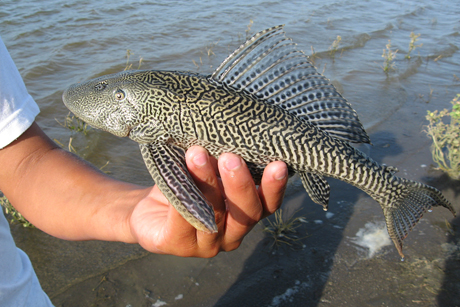
\includegraphics{MEImages/Pleco8-21.jpg}
\caption{\textbf{Fig.1.2 - A pleco caught in the Chacamax River in
Chiapas, Mexico - photo credit Krista Capps.}}
\end{figure}

\emph{To wrap this up, a photo of one of the invasive Loricariid catfish
mentioned earlier. More info on the system can be found at
\url{https://news.cornell.edu/stories/2013/08/freeing-pet-catfish-can-devastate-ecosystems}
. Can you think of how studying genomic diversity of these catfish - as
well as the source populations from which they come - could be useful?}

\emph{Resources cited in this section - I will typically cite in-line
actually}

Avise 2000

Ayres \& Grosberg (2005, \url{doi:10.1016/j.anbehav.2004.08.022})

Freeland, J. 2020.

Hahn, M.W. 2019.

Hedrick, P.W. 1995.

Templeton, A.R. (NCA era)

\begin{center}\rule{0.5\linewidth}{0.5pt}\end{center}

*** don;t forget the experiential stuff *** text: experiential appendix:
poppr, barcoding, rad data, etc I think what we have here is Chapter 1
is for first day of class, assign some reading to be discussed in week 2
of class. Chapter 2 easily encompasses some lecture, some Geneious, some
reading/discussion time and thus more than just 2 days of the class.

\hypertarget{sampling-the-simplest-genomic-data}{%
\section{2. Sampling the `simplest' genomic
data}\label{sampling-the-simplest-genomic-data}}

I'm going to start this text in a very different place than I've started
teaching this class before; I have tended to start at the beginning and
work through the history to reach the present. My efforts at
re-organizing my class in 2020 led me to see this as a funny choice. For
one, it means we may spend some time talking about methods that are
currently DOA, even if we learned a lot from them at the time. At this
point, there is simply no reason for me to re-hash AFLP markers (I won't
even define the acronym). Even the most in-vogue methods of 2020 will
not be as exciting in 5 years. But our efforts to learn this material
should be generic to the specific means of obtaining data, anyway.

Additionally, I've recognized that some applications of molecular data
have been treated as distinct, and separated in other texts or in
previous versions of my class, even though their basic methodology
aligns pretty clearly with understanding some simple basics about DNA
sequence data and how it evolves within and among populations of
biodiversity. I hope that is clear from this first data-focused chapter,
which itself raises some questions about how we observe and quantify
patterns of diversity in nature.

\begin{figure}
\centering
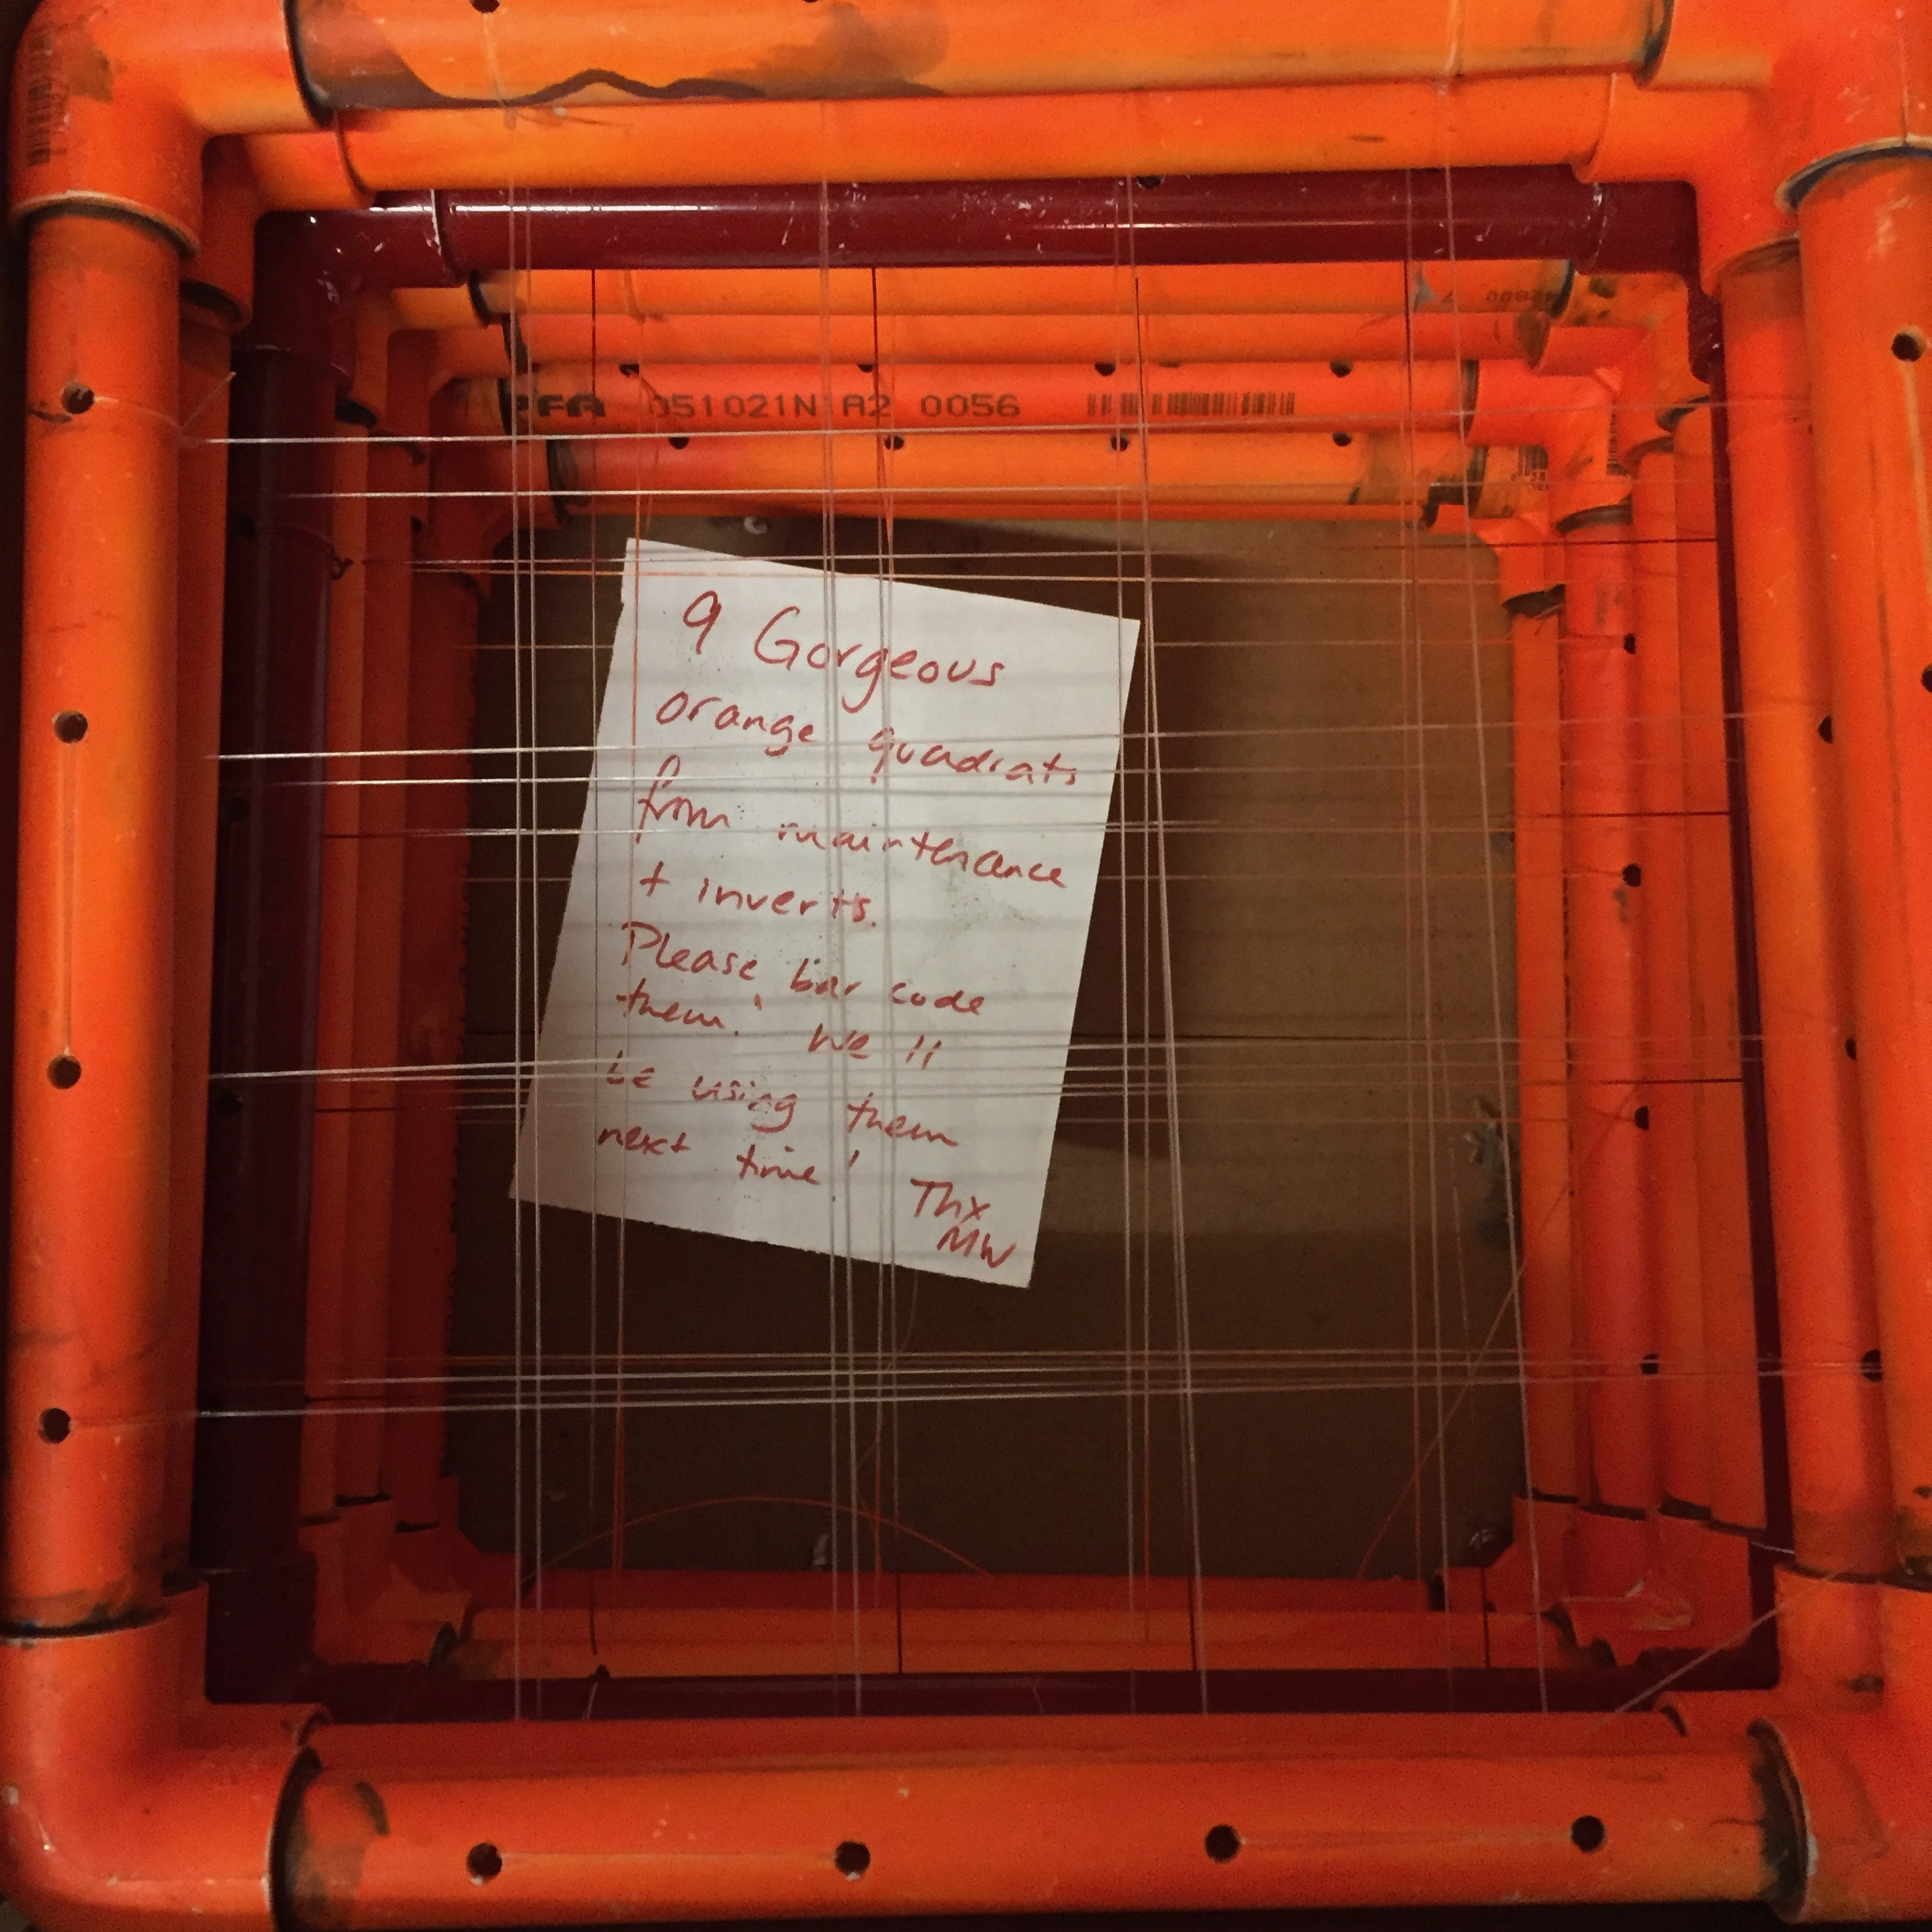
\includegraphics{MEImages/marsquadrats.jpg}
\caption{\textbf{Fig.2.1 - 9 gorgeous orange quadrats, photo credit J.
Wares but quadrats and note thanks to Dr.~Marjorie Wonham, I believe. }}
\end{figure}

\hypertarget{our-sampling-effort}{%
\subsection{2.1. Our sampling effort}\label{our-sampling-effort}}

If you aren't familiar with a \emph{quadrat}, the photo above (Figure
2.1) includes ``9 gorgeous orange quadrats'' and you may quickly deduce
that these are nothing more than PVC squares with grids installed using
heavy fishing line, and the whole thing spray painted orange so they can
be easily found in an intertidal marine habitat with sprawling
macroalgae and dark rock coves studded with limpets. A \emph{quadrat} is
a means to sample spatial diversity that is commonly used by ecologists
to estimate the diversity of a larger spatial domain, with the scale
varying depending on the system one is looking at, the evenness in that
system, and the type of diversity to be counted (and thus extrapolated
to say something about the whole ecosystem).

So, what I often tell my students is that if you wanted to characterize
the vegetation of your college campus, and you randomly tossed down a
single quadrat of this size (\textasciitilde25cm across), what would you
find? Maybe manicured lawn, maybe some flowering plants, maybe the root
system of a single tree. You know that wouldn't say much about the
vegetation on your campus, so you would want to think about how to gain
data from multiple quadrats before you made any characterization - and
you would want to think about how randomly they are used (Anne
Magurran's \emph{Measuring Biological Diversity} has some great insights
into this problem).

Similarly, a single random anonymous DNA sequence from your species of
interest may or may not represent well the genome as a whole, and may or
may not be appropriate to answer your question. But first, to keep
things simple, lets do exactly that. If you take a small sample of a
genome - perhaps a single gene, or locus, that can be easily captured
using modern molecular approaches like PCR or metabarcoding
(\protect\hyperlink{BoxB}{\textbf{BOX B:}} How molecular data are
obtained). That means that it is on the order of 100s of nucleotides in
length (long enough to capture variation in many instances), and we can
\emph{mostly} ignore biological recombination of this fragment (though
PCR itself can promote the formation of chimeric, recombinant sequences
- Katz et al.~2009)

(\emph{so now you can imagine having some DNA sequences from several
individuals - and we are thinking about the variation among those
sequences})

We are assuming that the same \emph{homologous} sequence(s) can be
obtained from other individual organisms or samples. In other words,
whenever we make comparisons of two DNA sequences, we assume that they
have a single common origin and the variation between them represents
the mutation events that have happened since that point of common
ancestry, whether we are comparing members of the same population or
individuals from divergent species. This itself can be difficult; the
more we know about genome structure, the more we know that many gene
regions are duplicated and lost through time, so that some gene regions
will have multiple, \emph{paralogous} copies in the same genome, and
counting the mutational events will be wrong if the contrast between
molecules is specified incorrectly.

\begin{figure}
\centering
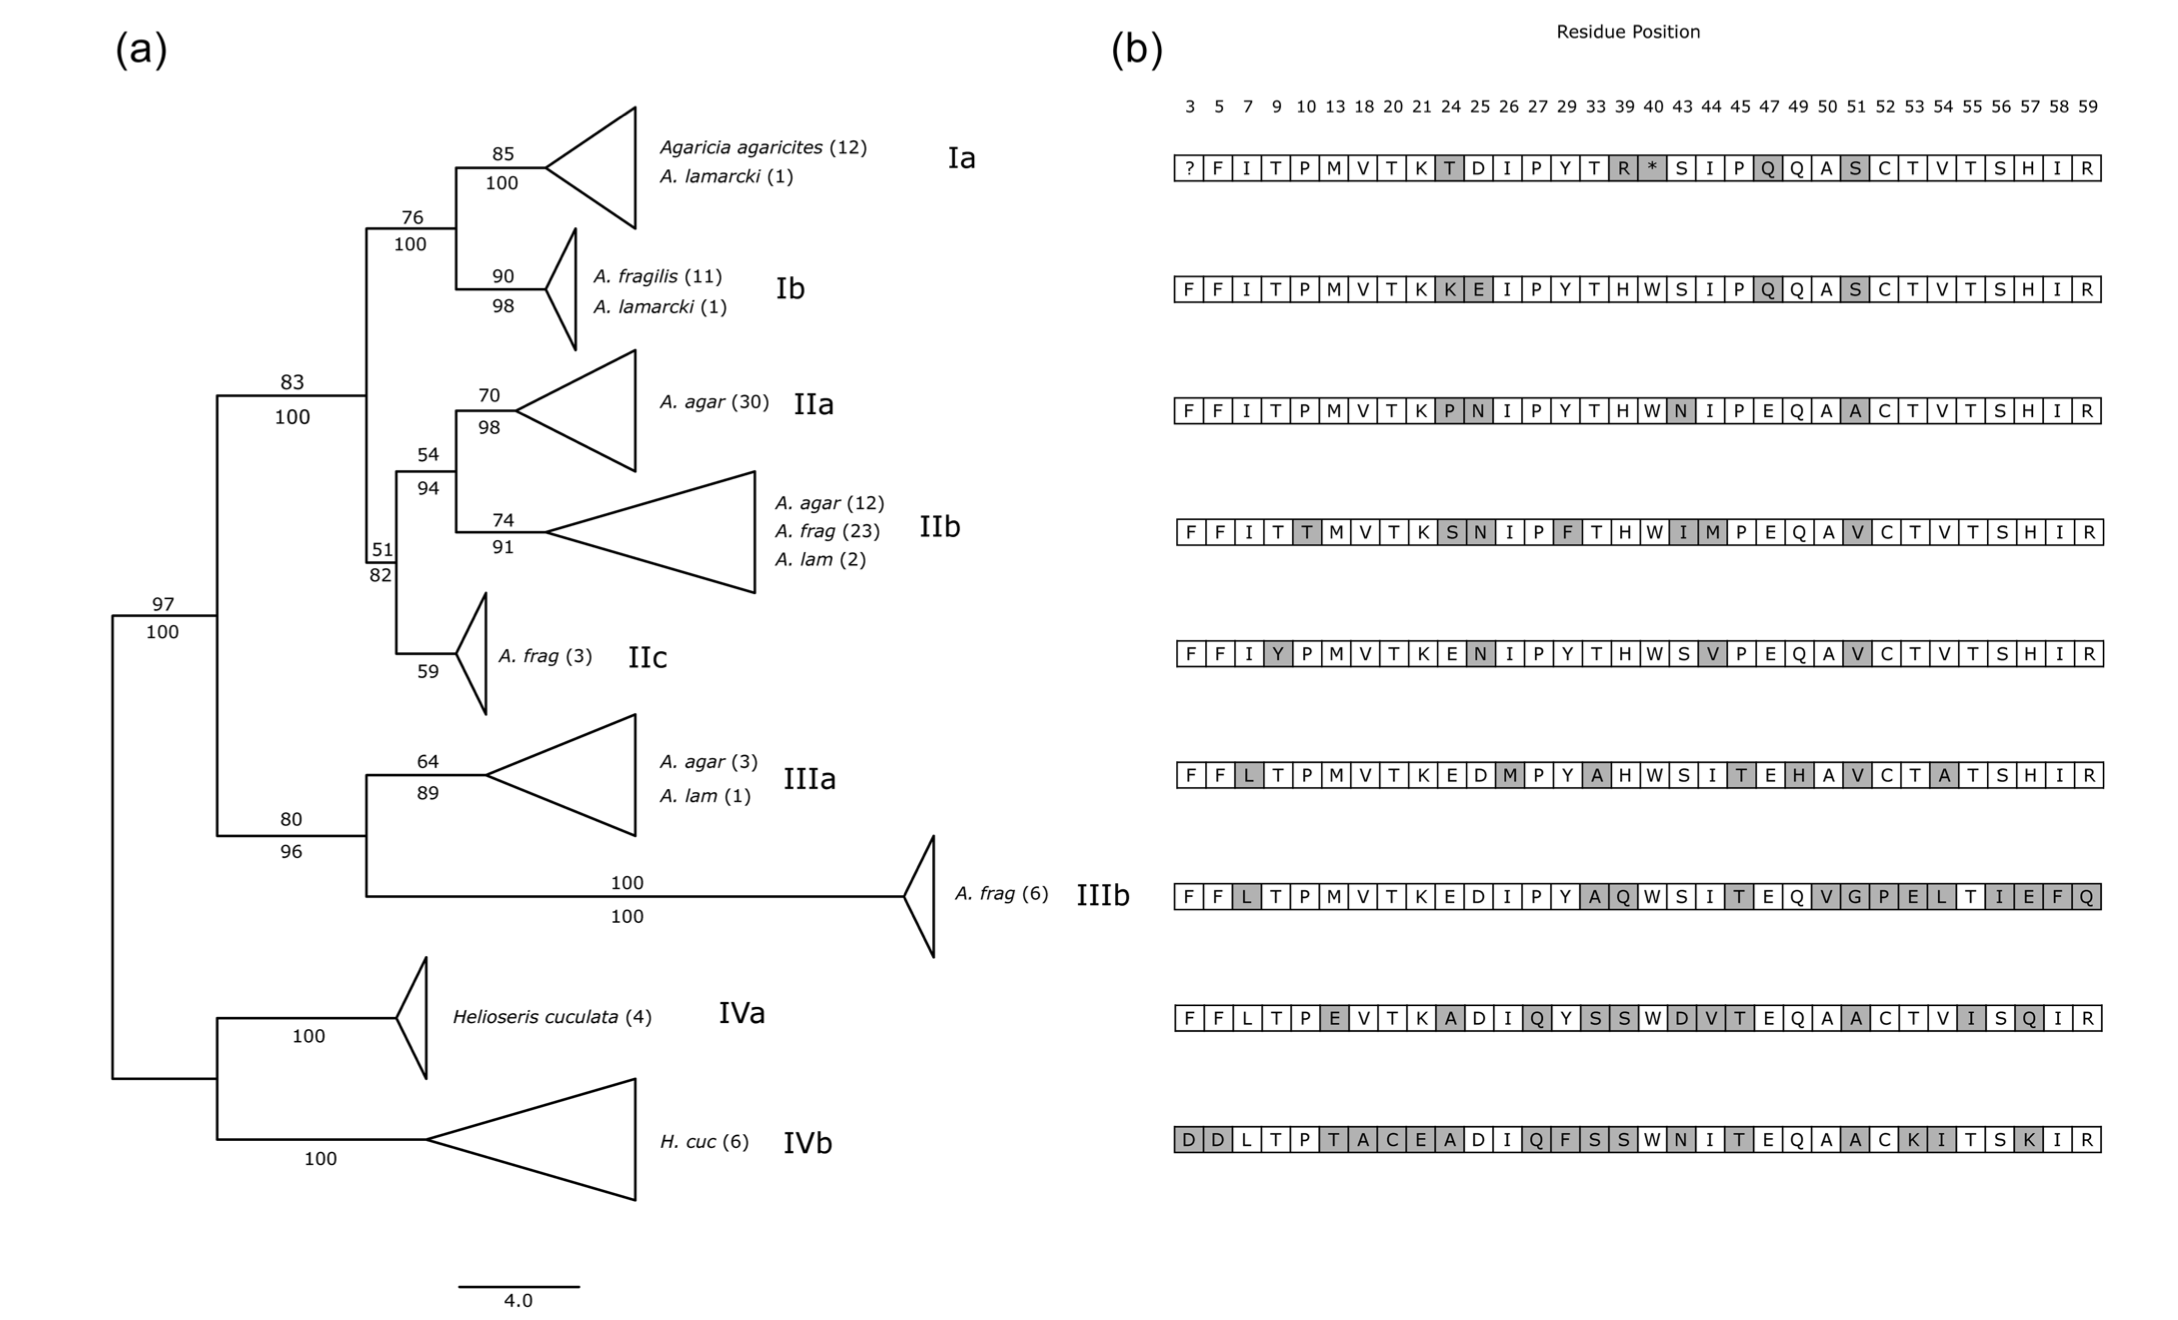
\includegraphics{MEImages/AgarFP.jpg}
\caption{\textbf{Fig.2.2 - The same PCR primers amplify allelic
(homologous) and distinct gene copy variation (paralogous) in
fluorescent proteins of the coral \emph{Agaricia}. Determining how to
separate this diversity for the typical analytical approaches in the
field of molecular ecology is not trivial in such cases. Note the
distinct amino acid sequences resulting from the sequence diversity; one
copy appears to be non-functional with a `stop' codon in the middle of
the domain. From Meyers, MK 2013 \emph{J. Heredity}
\url{doi:10.1093/jhered/est028}.}}
\end{figure}

The problem of gene duplication can include whole genomes (polyploidy is
common in plants, and has even generated new species in frogs) or just
parts of a genome, and depending on how recent the evolutionary event
was, it may be impossible to isolate parental-contributed diversity from
the diversity found across copies. However, there are ways to analyze
such data and we will discuss further as these instances come up.
\emph{For now we are only focusing on the gene sequences we can recover
to represent natural diversity, and how to compare those sequences (not
worrying about the combinations of copies within an individual).}

In addition, we assume that the individual nucleotides (A,C,T,G) in
these DNA sequences being compared are homologous. This means
\emph{aligning} the sequences so that the variation we see in a single
position - some sequences have a C, others have a T, for example -
represent a single mutational event (more on this assumption later)
rather than inadvertently comparing haphazard parts of that gene region.
In Figure 2.3, a DNA sequence for a protein-coding region provides an
example where it is clear that despite some nucleotide variation, each
DNA sequence is coding for the same amino acid sequence. It would be
unusual for so much similarity to exist among distinct genomic regions
(though biology can throw plenty of improbable curveballs, some of them
noted above), and we can evaluate this probabilistically (Altschul et al
1990).

\begin{figure}
\centering
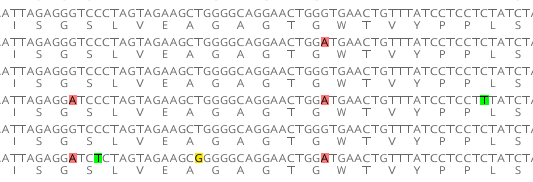
\includegraphics{MEImages/DNAalign.jpg}
\caption{\textbf{Fig.2.3. DNA sequence alignment, with amino acids shown
for protein sequence. The colored positions indicate mutational
diversity where the less frequent variant is highlighted.}}
\end{figure}

Once these steps are complete - DNA sequences obtained from comparable
parts of the genome, and aligned so that the mutational events are clear
- we can start to make some simple assumptions about what the diversity
among sequences means.

\hypertarget{genetic-distances-and-barcode-gaps}{%
\subsection{2.2 Genetic Distances and `Barcode
Gaps'}\label{genetic-distances-and-barcode-gaps}}

From the DNA sequences in Figure 2.3, we can start making one of the
first and most basic assessments of genetic distance between sequences
or between collections of sequences. For example, the comparison between
sequence 1 and sequence 2 (counting from the top) shows a single
nucleotide difference between them (an A/G transition), out of 63 such
site comparisons. If you are unfamiliar with how these data are shown,
the nucleotide sequence includes only (A/C/T/G), and below each
amino-acid-coding triplet the amino acid single-letter code is shown; in
many cases we would compare sequences that are not protein coding (or
for which we don't care about the product) and so the amino acid
sequence would not be shown.

From these data, we can estimate the distance \emph{d} based on this
proportion of differences between sequences, e.g.~\emph{d} = 1/63 =
0.0159. Then, comparing sequence 1 to sequence 3 there are no
differences, so \emph{d} = 0; and sequence 1 to sequence 4 represents
\emph{d} = 3/63 or 0.0476. You should be able to make similar
calculations for all pairs of sequences in Figure 2.3. The R code below
shows how to turn those genetic distances into a very basic histogram.

\begin{Shaded}
\begin{Highlighting}[]
\NormalTok{dist1}\OtherTok{\textless{}{-}}\FunctionTok{c}\NormalTok{(}\FloatTok{0.0159}\NormalTok{,}\DecValTok{0}\NormalTok{,}\FloatTok{0.0476}\NormalTok{,}\DecValTok{0}\NormalTok{,}\FloatTok{0.0635}\NormalTok{,}\FloatTok{0.0159}\NormalTok{,}\FloatTok{0.0317}\NormalTok{,}\FloatTok{0.0159}\NormalTok{,}\FloatTok{0.0476}\NormalTok{,}\FloatTok{0.0476}\NormalTok{,}\DecValTok{0}\NormalTok{,}\FloatTok{0.0635}\NormalTok{,}\FloatTok{0.0476}\NormalTok{,}\FloatTok{0.0476}\NormalTok{,}\FloatTok{0.063}\NormalTok{)}
\FunctionTok{hist}\NormalTok{(dist1,}\AttributeTok{breaks=}\DecValTok{4}\NormalTok{,}\AttributeTok{col=}\StringTok{"darkred"}\NormalTok{)}
\end{Highlighting}
\end{Shaded}

\includegraphics{ASU_MolEcol_UNshiny_files/figure-latex/bargap1-1.pdf}

Now all of these pairwise distances are shown in a histogram, above, and
in this case all of those sequences come from organisms sharing the same
Latin binomial, \emph{Chthamalus fragilis} (though later in this unit
you will see it is more complicated than that). Imagine comparing these
sequences with the sister species, \emph{C. proteus}, by adding just a
single additional set of comparisons between the 6 sequences above and a
single one from \emph{C. proteus}. The contrast can further be
identified in our R histogram by coloring the bars in order; note the
change in scale on the x-axis as we add more distantly related
sequences. Yes, \textbf{R} friends, I know it can be done more
efficiently. Bear with me, this section is basically unedited since I
wrote in April 2020 as my class flipped to online during the beginning
of \textbf{COVID}, but I want it to be clear where the outputs come
from!

\begin{Shaded}
\begin{Highlighting}[]
\NormalTok{dist2}\OtherTok{\textless{}{-}}\FunctionTok{c}\NormalTok{(}\FloatTok{0.0159}\NormalTok{,}\DecValTok{0}\NormalTok{,}\FloatTok{0.0476}\NormalTok{,}\DecValTok{0}\NormalTok{,}\FloatTok{0.0635}\NormalTok{,}\FloatTok{0.0159}\NormalTok{,}\FloatTok{0.0317}\NormalTok{,}\FloatTok{0.0159}\NormalTok{,}\FloatTok{0.0476}\NormalTok{,}\FloatTok{0.0476}\NormalTok{,}\DecValTok{0}\NormalTok{,}\FloatTok{0.0635}\NormalTok{,}\FloatTok{0.0476}\NormalTok{,}\FloatTok{0.0476}\NormalTok{,}\FloatTok{0.063}\NormalTok{,}\FloatTok{0.16}\NormalTok{,}\FloatTok{0.17}\NormalTok{,}\FloatTok{0.16}\NormalTok{,}\FloatTok{0.17}\NormalTok{,}\FloatTok{0.17}\NormalTok{,}\FloatTok{0.18}\NormalTok{)}
\NormalTok{hiscols}\OtherTok{\textless{}{-}}\FunctionTok{c}\NormalTok{(}\StringTok{"darkred"}\NormalTok{,}\StringTok{"darkred"}\NormalTok{,}\StringTok{"darkred"}\NormalTok{,}\StringTok{"darkred"}\NormalTok{,}\StringTok{"lightblue"}\NormalTok{,}\StringTok{"lightblue"}\NormalTok{,}\StringTok{"lightblue"}\NormalTok{,}\StringTok{"lightblue"}\NormalTok{,}\StringTok{"lightblue"}\NormalTok{)}
\FunctionTok{hist}\NormalTok{(dist2,}\AttributeTok{breaks=}\DecValTok{8}\NormalTok{,}\AttributeTok{col=}\NormalTok{hiscols)}
\end{Highlighting}
\end{Shaded}

\includegraphics{ASU_MolEcol_UNshiny_files/figure-latex/bargap2-1.pdf}

Now, we have recapitulated what is called the `barcode gap', a classic
figure below (2.4) from Meyer \& Paulay (2005,
\url{https://doi.org/10.1371/journal.pbio.0030422}). What this is
suggesting is that though there is variation within species (in
phenotype as well as sequence divergence), in many cases that variation
is considerably less than the distinctions from other species (also
known as distinct populations that are demographically isolated in some
way).

\begin{figure}
\centering
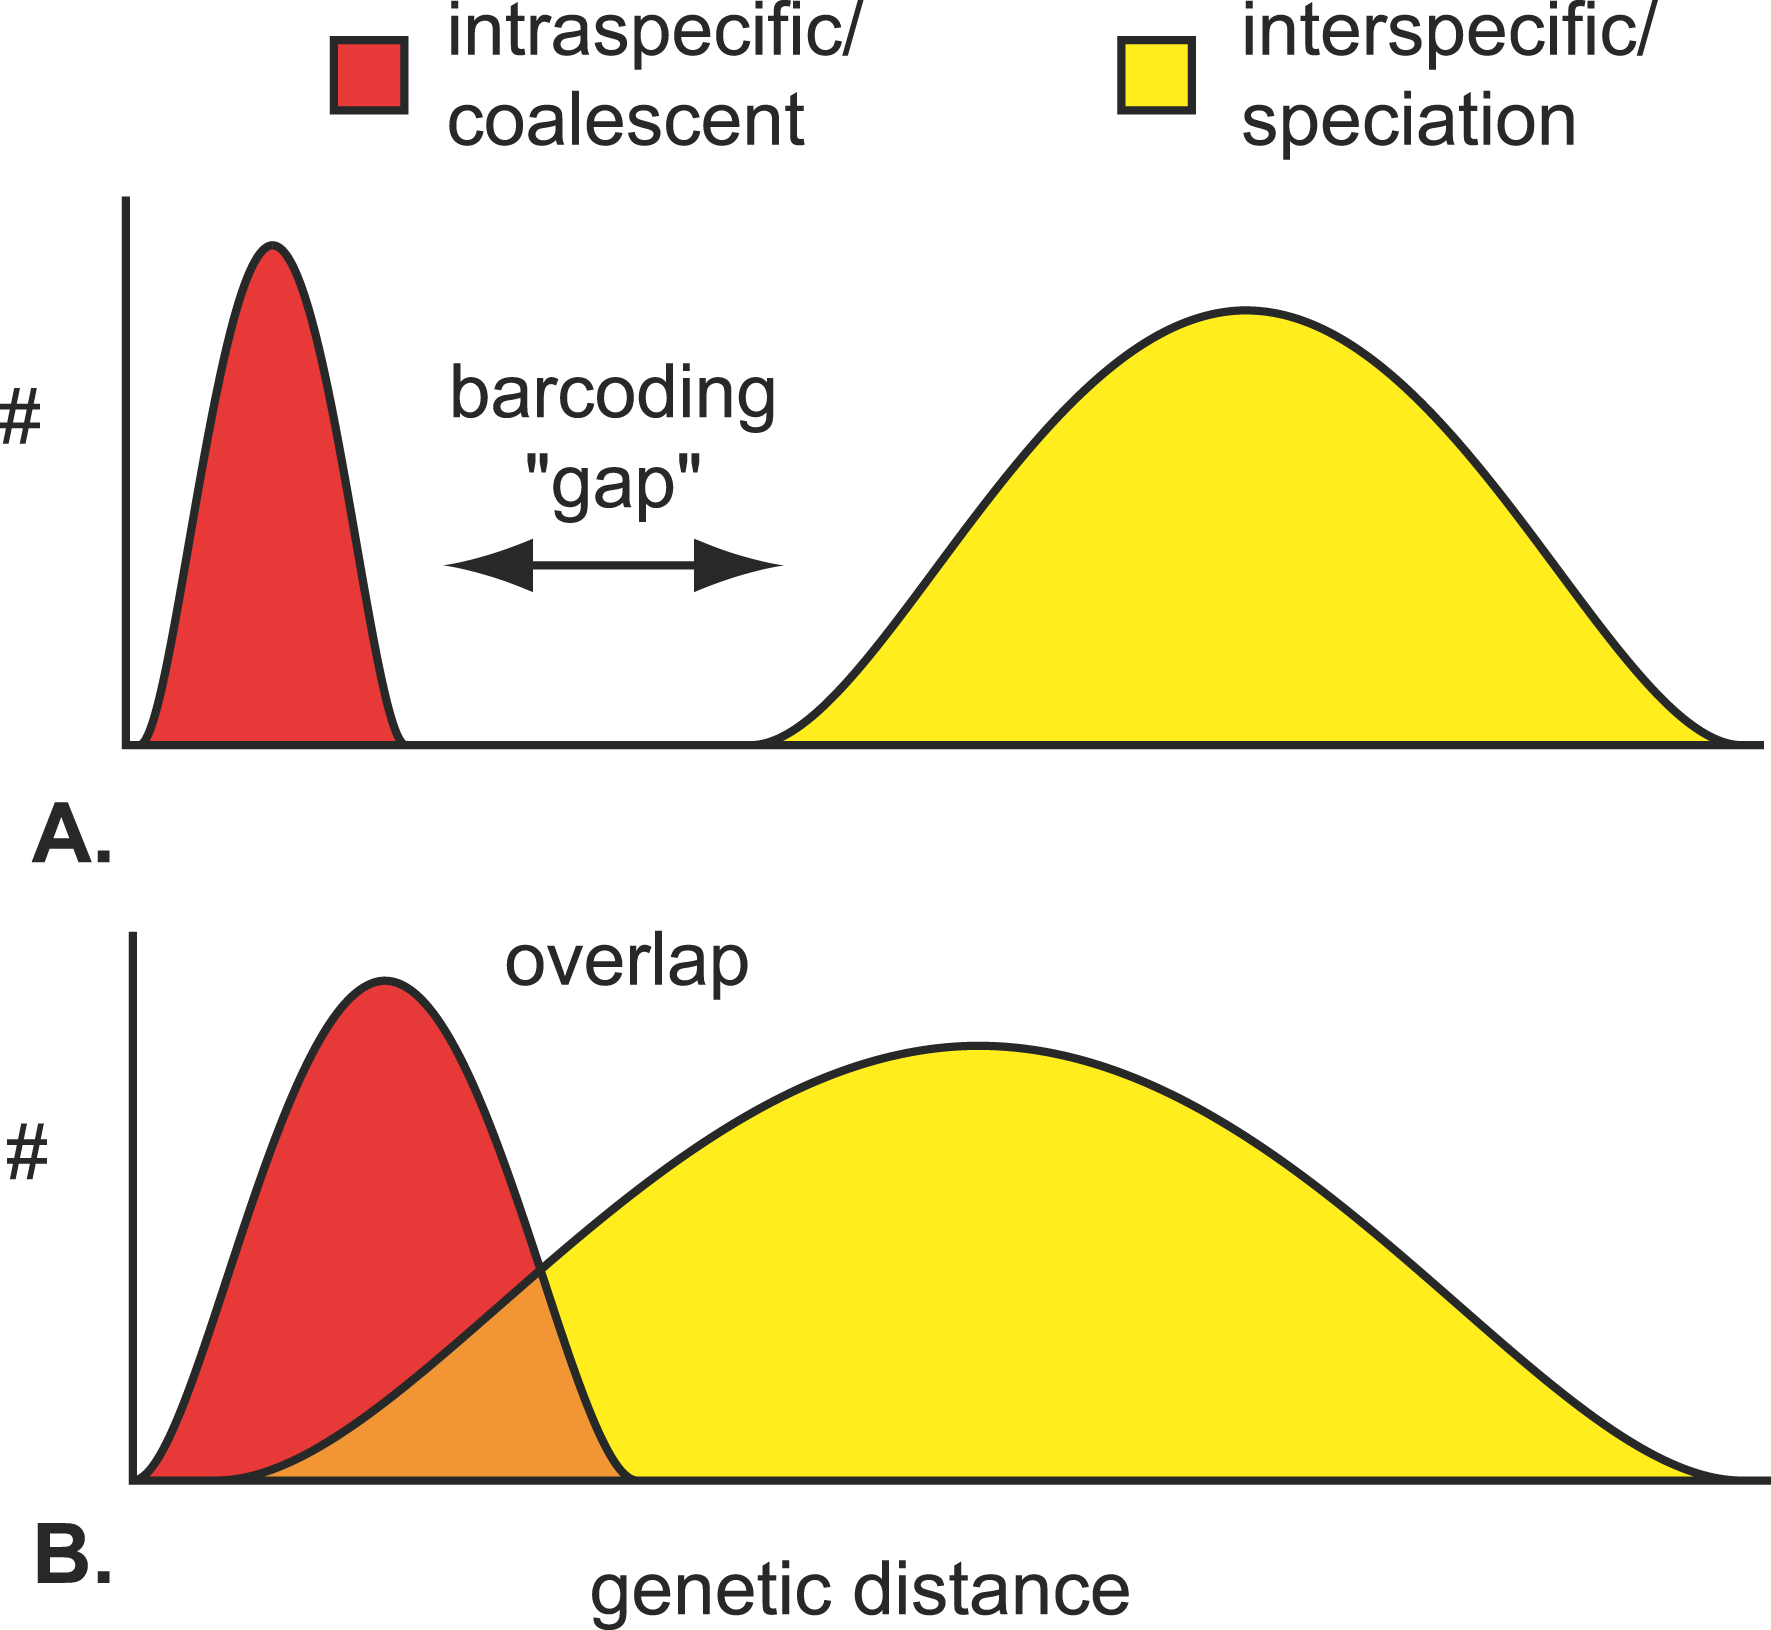
\includegraphics{MEImages/MeyerPaulaygap.jpg}
\caption{\textbf{Fig.2.4. Illustration of the idealized barcoding gap
(top panel) for contrasting diversity within and between species; the
bottom panel shows that sometimes it gets more complicated. Just ask
folks who study corals\ldots e.g.~Tonya Shearer's work.}}
\end{figure}

Why are we exploring this kind of diversity among DNA sequences? Well,
our first goal as molecular ecologists may be simply to evaluate the
distribution and abundance of diversity in and among sampled habitats.
We can use the sequence data itself to identify \emph{what} is found in
a habitat, when this is a more effective approach than other forms of
identification. For reasons that will become clearer as we learn more
about the different modes of inheritance (natural history!) of gene
regions, the ``barcode gap'' is most effectively evaluated with genes
that (1) exhibit high mutational diversity, (2) are haploid, and (3) are
uniparentally inherited; but it will work for any gene that provides
sufficient resolution. For this reason, mitochondrial and chloroplast
loci are often the first tools used for such surveys.

(note to flesh out: Microbial and barcode gap tend to rely on haploid
low recombination otherwise complete dna so we start here for
comparing.)

\textbf{Example 1. Some aspects of the focal diversity are well
characterized.}

If we assume that the species are identifiable (at one life stage or
another), and there is clearly greater genomic divergence between
different species than between different individuals of the same species
(the ``barcode gap''), then with a reference library of representative
individuals for each species we can use DNA sequencing to identify
remaining unknown or hard-to-identify specimens. A great example comes
from Katie Bockrath's dissertation work on freshwater mussels
(Unionidae). Though many freshwater biologists will laugh to read this
sentence: lets assume that the adults can be clearly identified, sorted
into species, and DNA can be sequenced from those individuals. Our real
challenge lies with the larvae and the juveniles, which are themselves
miniscule (hundreds of \(\mu\)m). Unionid mussels produce larvae
(glochidia) that are obligate parasites on fish gills; they must
developmentally transform on a fish to mature to the juvenile stage,
when they are still quite small but drop off into the sediment to
continue maturation.

There are a lot of complexities involved in this life cycle, and
knowledge of which species are host-generalists versus specialists, that
are beyond the question addressed here. However, Dr.~Bockrath wanted to
know \emph{which} mussel species are using \emph{which} fish species as
hosts, which itself can influence how well individuals move via their
host and how sustainable a population may be. In order to do this, fish
gills were sampled for glochidia and the tiny (5-10mg) tissue samples
collected. To ensure that PCR reactions are specific to the mussel and
not the fish, Katie used her knowledge of the quirky life history of
Unionids to target a relatively unique coding region in the
mitochondrial control region (FORF; Breton et al.); this means that her
PCR would not amplify fish DNA, only mussel DNA.

Because of the `barcode gap' between the diversity found within a
species, e.g.~\emph{Toxolasma pullus} and the diversity found in other
species (or other genera) like \emph{Elliptio icterina}, Katie was able
to assign each tissue sample - as minute as it was, and intermingled
with fish gill tissue - to the species that is able to use that
particular fish species as a host. In this way, molecular techniques can
be used to identify species interactions and the specificity of those
interactions - and very similar approaches are used when there is a need
to identify parasites or pathogens throughout nature. It does, however,
require that a reference library of data are available and easily
searched for a likely match and high sequence similarity with the
`query' sequence. In some cases, a researcher must collect and generate
such a database for local diversity themselves; in other cases,
representative diversity is already available at the NCBI
sequence/genome database called ``GenBank''.

\textbf{HERE PUT A SHORT MODULE ON THE MATHEMATICS OF BLAST AND
AVAILABLE DATA, WHEN IS THE E-VALUE USEFUL AND WHEN YOU NEED OTHER
INFORMATION}

\url{https://www.ccg.unam.mx/~vinuesa/tlem/pdfs/Bioinformatics_explained_BLAST.pdf}

\textbf{LETS LOOK AT EXAMPLES USING GENEIOUS}

A major shift in recent years in how environmental samples are analyzed
for the presence of particular diversity revolves around the cost of
data acquisition. Particularly when dilute resources like river water
are being evaluated, it has been cost-effective to design \emph{very}
specific primers for a target organism (and target gene region) such as
a rare or threatened fish, and use \emph{quantitative PCR} to localize
where samples come from that contain positive responses to these assays.
As the cost of sequencing continues to decrease, more and more studies
are asking about the presence of focal species' DNA amidst the noise of
the DNA from many other organisms in the environment; an active area of
study is how to minimize false positives (and false negatives) in qPCR
approaches as well (BOX X: ENVIRONMENTAL DNA).

\emph{this is an example of a `closed reference' library. in more
complex scenarios, diversity that was not \textbf{ a priori } known will
be missed in such instances, so either de novo or open referenCe
libraries should be used. our search for diversity depends on how we ask
the question!} will also want to talk about OTUs vs exact sequence
variants later when we have fully grasped DNA barcoding and the barcode
gap

\hypertarget{BoxX}{%
\subsection{Box A. Environmental DNA}\label{BoxX}}

The exploration of ``environmental DNA'' in the past decade or so has
seen remarkable growth (Cristescu \& Hebert 2018,
doi.org/10.1146/annurev- ecolsys- 110617- 062306). Essentially, there
are two significant components to such work. First, how to effectively
collect, concentrate, and isolate DNA from diverse environmental samples
including ocean water, soil, rivers, or points of organismal contact.
This often means taking highly dilute samples that may include tissue or
cells, fecal matter, saliva, blood or gametes that represent the
(recent) presence of an organism.

Second, the effort towards collecting, concentrating, and isolating that
DNA so that it can be identified has to meticulously avoid the potential
for contamination from other point sources, including the equipment that
has been used previously, the investigators themselves, etc. The genomic
target, regardless of focal species, is often the mitochondrial genome
because it is present in so many copies per cell, relative to the
typical two copies for nuclear loci.

Third, consideration must be given as to whether it is more
cost-effective for a particular question to use a `metabarcode' approach
or other high-throughput method for evaluating the diversity of a
sample, or a targeted approach that must be effective not only in
identifying the presence of a particular species but also in excluding
amplification of taxa with similar DNA sequences in the target region.
Congeneric or confamilial species are a good example, because the
primers used in PCR or qPCR do not have to be perfect matches to have
the potential to amplify. Remember that tens of thousands of different
metazoans have been amplified and sequenced using one particular pair of
primers for the mitochondrial COI region! (Folmer et al.~1994) One study
(Wilcox et al 2013, \url{doi:10.1371/journal.pone.0059520}) developed
primer/probe sets for qPCR to detect non-native \emph{Salvelinus} amidst
congeneric and confamilial species; their work showed a greater effect
of finding divergent regions for primer design than for the fluorescent
probe, and the mismatches being near the 3' end of the primers tending
to add to the specificity. Putting thought and experimentation into
early testing of eDNA methods is absolutely critical for avoiding
misinterpretation of results.

Fourth, a sampling strategy has to take into account the life history of
the organism as well as other features of its biology. Are there
spawning aggregations that affect how the environment would be sampled?
Is it a hard-shelled crustacean that may only leave traces in the
environment during molting or defecation (Anderson et al 2020)? The
shedding of DNA, as well as its persistence in the environment (the
`decay rate') are active fields of study with respect to how
temperature, UV exposure, and flow of the environment are all critical
to answering such questions. There has also been intriguing work done to
ensure the specificity of some eDNA/metabarcoding work to the
association with a target organism. In some cases, nearby environments
must be sampled to `subtract out' baseline environmental diversity; in
others, targeted swabbing of tissues can be used to avoid that
environmental diversity. van Zinnicq Bergmann et al (2021,
\url{https://doi.org/10.1111/1755-0998.13315}) were able to assess the
diets of juvenile bull sharks by quickly swabbing the fecal residues
from inside a shark's cloaca without contamination of surrounding
seawater diversity. This paper spends less time talking about how one
actually manages to swab the cloaca of a shark, likely presenting
distinct challenges.

Finally, the field of `environmental DNA' is of course about actually
getting those answers in robust ways. What diversity is present - does
it match the diversity found using other types of collection protocols
or gear? Does it save effort over those other methods, is it more
specific? Does the diversity respond to shifts in the environment? Can
the rare species be found, or the symbiont diversity identified? These
are remarkable times for studying diverse ecological questions, and they
(mostly) involve the exact same methods of matching observed DNA
sequence data from a sample with prior understanding from known
organismal diversity.

\textbf{For our reading group this week, we will consider how
metabarcoding methods are used to identify the pollen gathered by bees
in Bell et al.~(2017) \url{doi:10.3732/apps.1600124}. This example does
not involve the concerns of `concentrating' target DNA from the
environment as it does with inferring the presence of organisms that
remain unseen, but is still a useful example.}

\textbf{Example 2. Diversity is (partly) well characterized, and must be
sorted from sequence data.}

As the cost of sequencing has dropped, an equally common type of
environmental study using molecular data are what may be referred to as
`metabarcoding' studies (distinguishing from `metagenomic' in which
shotgun sequencing of - for example, microbes - is intended to tell us
about the functional gene representation in a sample rather than the
identities of the microbes, an approach sometimes referred to as
\emph{reverse ecology}). This means that environmental samples are
stabilized for genomic analysis, and then the sequence region to be
compared is amplified from the environmental sample - amplifying much of
the diversity found within. This might be a soil sample, a liter of
ocean water, or the homogenized tissues fouling a dock. The genomic
region chosen has to be considered relative to the diversity being
studied, whether microbes or fungi or root hairs or metazoans. Remember:
\textbf{the natural history of the gene region, as well as the natural
history of the organism!}

The distinction with the mussel example is that rather than sequence
tissues one at a time (the Sanger sequencing method, see
\protect\hyperlink{Box1}{\textbf{BOX 1:}}), they are typically not able
to be separated and so must instead by sorted out after sequencing many
PCR amplicons either using old-fashioned cloning (labor-intensive and
expensive, plus requires Sanger sequencing) or high-throughput
sequencing (expensive but efficient; requires bioinformatic expertise
and effective design of identifying oligonucleotides that can be built
into the primers or adapters, see Bayona-Vasquez et al 2019, Hamady et
al 2008). Some questions require more conserved parts of the genome - as
with using ribosomal regions to barcode life - and some will require
much more variable regions to distinguish diversity. The trade-off
between regions of the genome that are constrained from varying (for
example, do you use the nearly-universal 18S ribosomal region that
varies rarely within species? Or the 16S ribsomal region that may pick
up cryptic diversity?) and this resolution of diversity (to the species
level or to unrecognized diversity, as with many uses of protein-coding
genes on metazoan mitochondria) is a good reminder that molecular
techniques are analogous to fishing gear. Different gear (rod and reel,
how fine is the net, is an electroshocker backpack being used, are you
kick-seining or casting a net) will influence what diversity you
capture, as will your skill with that gear.

Once again, these approaches are most useful for when diversity is very
difficult to characterize because of size, abundance, or ability to
capture. Bacteria have been a frequent target for this kind of approach
because the vast majority of bacteria cannot be easily cultured, but
deep sequencing (these days, through PCR amplification and multiplexed
sequencing on a high-throughput sequencing machine like an Illumina) of
the ribosomal 16S region (or one of the variable short sections within
it) will tend to generate a large number of comparable (homologous)
sequences that can be categorized based on their \emph{similarity} to a
reference library of bacterial species or genera. In this case, of
course we may find diversity that has not been previously catalogued,
and new diversity is identified in nearly every such study.

\begin{figure}
\centering
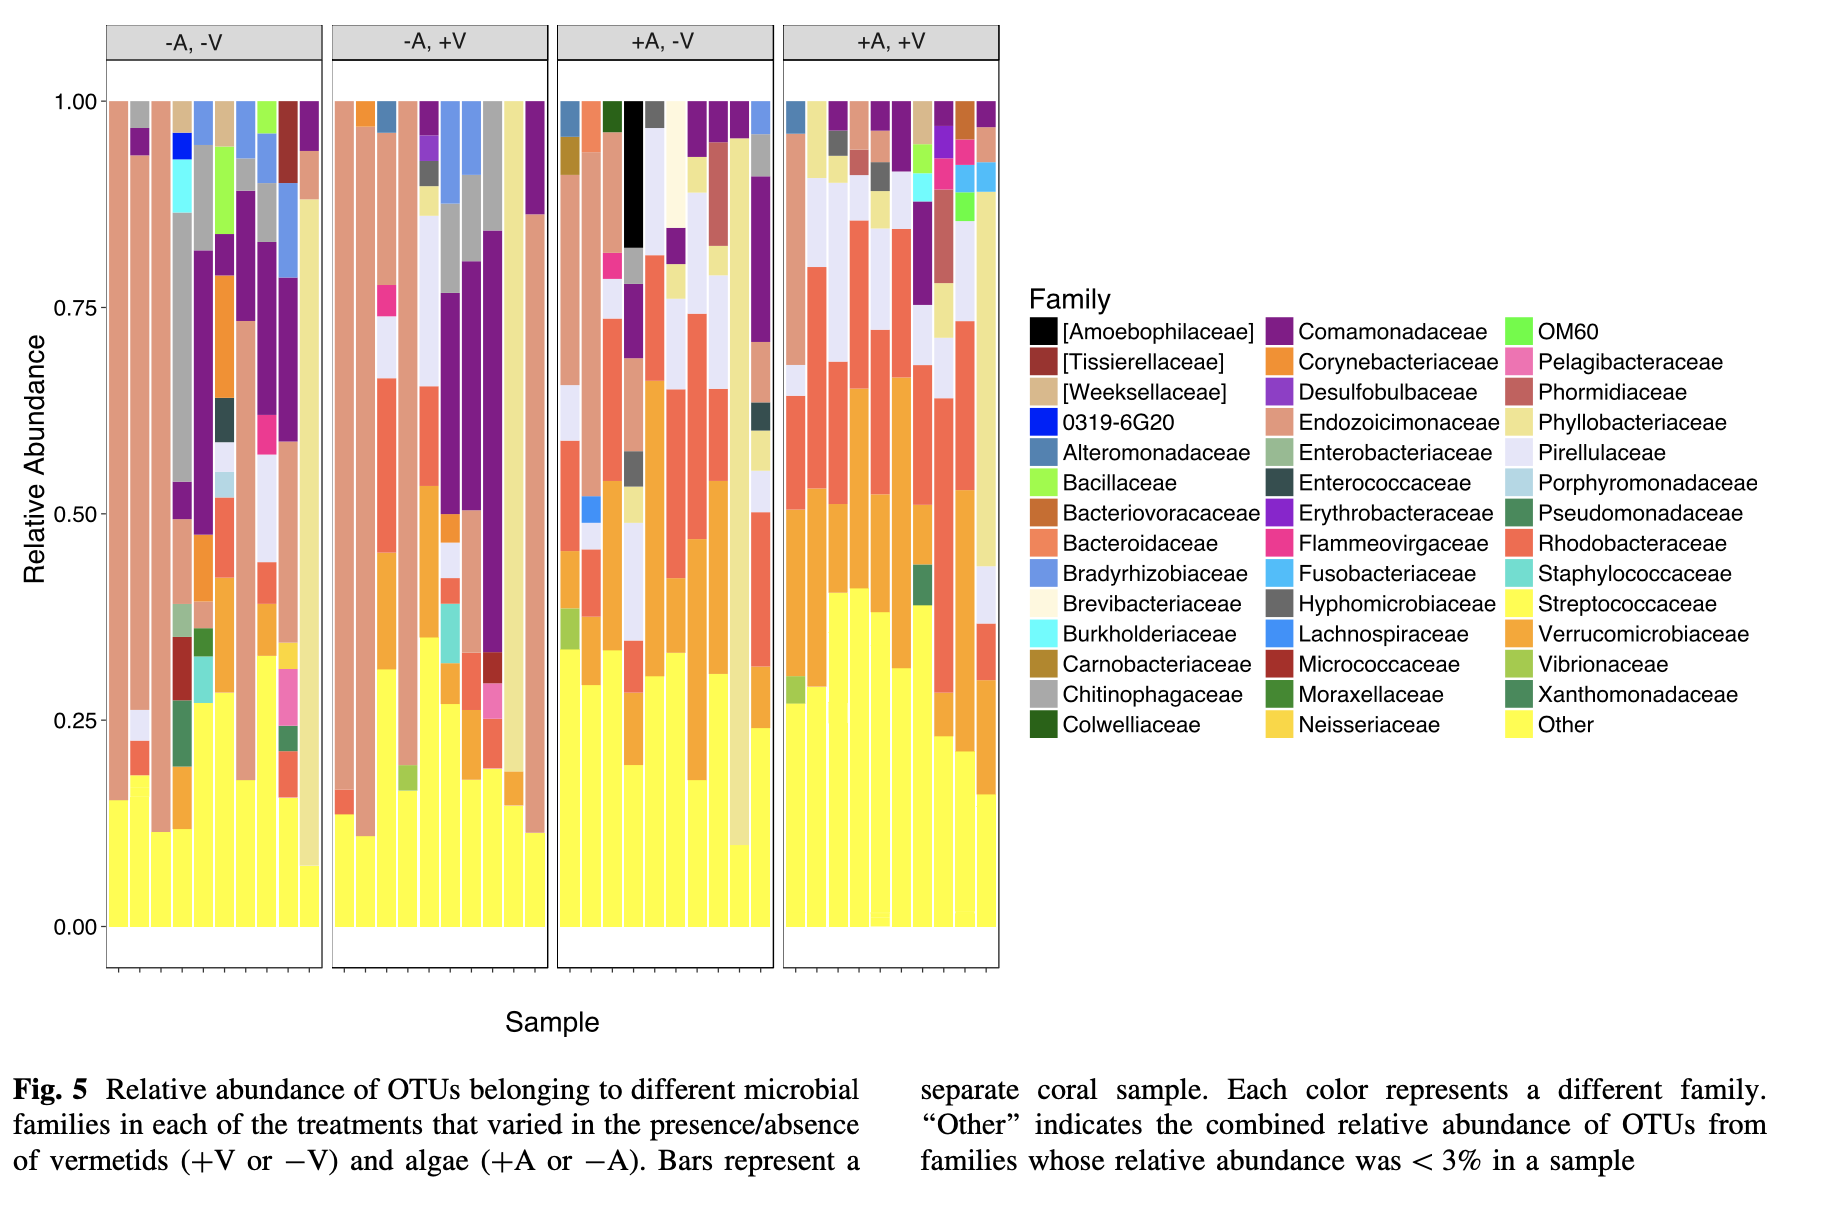
\includegraphics{MEImages/Brown2019Fig5.jpg}
\caption{\textbf{Fig.2.5. The distinct microbial communities, shown
using proportional color plots by individuals and by treatment, exhibit
some variation among coral colonies when either algal turf or vermetid
gastropods are present. From Anya Brown et al (2019) \emph{Coral Reefs}.
This case exhibits only slight variation among environmental treatment,
which is why we will consider quantitative approaches to distinguishing
samples or treatments in the next chapter and further in this text.}}
\end{figure}

The questions we may then ask include: how many distinct species in a
sample? Is it higher diversity in one treatment or location than the
other? Are the relative abundances of species the same in each of my
samples, or do they vary in interpretable ways? (Mind you, if you aren't
a microbiologist you may have a hard time knowing \emph{why} different
OTUs (operational taxonomic units, the sort-of-equivalence to species in
bacteria and Archaea) These questions require numeric or quantifiable
measurements and will be addressed in the next unit.

\textbf{Example 3. Further partitioning diversity, beyond taxonomy.}

Where we eventually will become fluent in this class is in recognizing
that our taxonomy - no matter what group of life you study - often does
not reflect the true diversity of life very completely. It is extremely
common to find that there are genomic distinctions among different
spatial samples of the same species, and that these distinct populations
represent variation in physiology, function, or other types of
ecological interaction. As we begin to consider how organismal diversity
responds to a warming planet, it has been tempting to think that
\emph{species} are gradually shifting to more poleward latitudes, for
example. However, in many cases it is far more accurate to recognize how
distinct \emph{populations} vary in environmental tolerance and their
ability to either move, adapt, or acclimate (Kelly et al.~2012).

The sequence data shown earlier from the barnacle \emph{C. fragilis} are
a good example of this. The overall divergence of sequences
\emph{within} this species are somewhat larger than typical for a
metazoan, though still very distinct from the sister species \emph{C.
proteus}. However, if we collect enough DNA sequence data - in this case
a common mitochondrial barcode region used in many metazoan studies, the
Folmer COI fragment noted in Box 1 - we may see that the genetic
distances among those DNA sequences easily group the individuals into 3
evolutionarily distinct lineages (Figure 2.5; Govindarajan et al 2015).
In many ways this is only different in the sampling strategy from the
microbial work mentioned earlier; we are asking ``what is where''
through sequencing (in this case, Sanger - individuals sequenced for a
single gene are still done most effectively this way), and the sequences
may identify new groups that are ecologically relevant or indicate
intrinsic diversity in ecophysiology that are not reflected by the name
of the species. Microbes on a coral, fungi in the forest, barnacles
along a coastline - we know where they are in a general sense, but the
specifics can tell us about functional and taxonomic diversity at a
finer resolution.

\begin{figure}
\centering
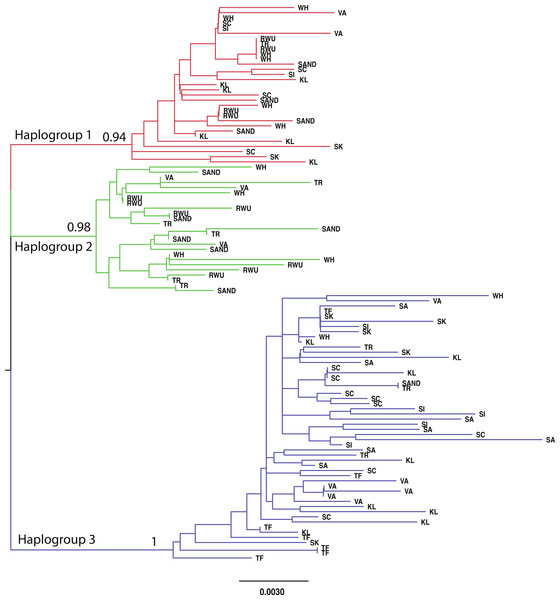
\includegraphics{MEImages/fig-1-1x-2.jpg}
\caption{\textbf{Fig.2.5a. A gene tree representation of the sequence
similarity among mitochondrial sequences sampled from the barnacle
Chthamalus fragilis on the east coast of North America.}}
\end{figure}

\begin{figure}
\centering
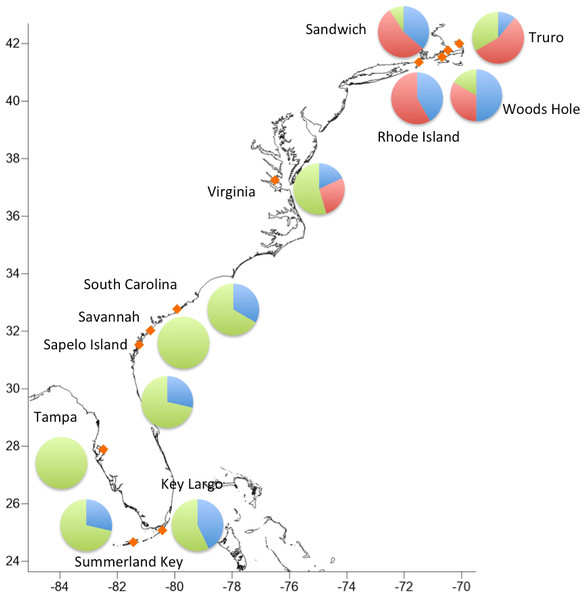
\includegraphics{MEImages/fig-3-1x-3.jpg}
\caption{\textbf{Fig.2.5b. Spatial distribution of distinct phylogenetic
clades shown in Fig.2.5a.}}
\end{figure}

This gene tree pattern (reflecting overall similarity of sequence,
though the models for inferring these relationships can be
mathematically complex in trying to estimate actual mutational
difference among sequences) raises many questions, many of which will be
addressed further as we gain skills in exploring the variation among
sequences under expectations of single, randomly-mating populations in
later chapters. However, by plotting WHERE each sequence was found you
can start to assess that the diversity is not randomly distributed - the
`red' type of diversity is only found in the northern part of the range
(Fig 2.5b). This appears to be an example where some diversity is more
likely to be found in certain parts of the distributional
(environmental) range of this species - suggesting variation in
environmental tolerances or performance. To quantify this variation
requires additional approaches, and to explore this hypothesis of local
adaptation will require additional experiments.

By the way, if you were really paying attention as we plotted the
barcode distances within \emph{Chthamalus} above, you may have noted
there was already a barcode gap - it just corresponds to a finer scale
than recognized ``species''! In the next unit, we will start to explore
how ecologists and geneticists have somewhat independently identified
similar approaches to measuring and distinguishing the diversity from
distinct spatial or environmental samples, and will note where
specialized metrics are necessary.

\emph{For your exercise this week}, we will (a) learn how to use the
free software Geneious at a basic level; (b) download DNA sequence data
for a group of organisms of your choosing (roughly 8-10 sequences per
species for 4-5 related species is a good size); (c) align the sequence
data (we will do this in class); (d) use the resultant distance matrix
data to plot your own ``barcode gap'' histogram (\emph{with more
guidance on how to use the R code above}) and ask how well this model of
interindividual and interspecific divergence applies to the
\emph{taxonomic} diversity of your chosen group of organisms - what are
the reasons it might not, and how could this understanding be applied to
a question of distribution, abundance, or interactions?

\emph{We will also take some class time to discuss the `reverse ecology'
approach mentioned in the Marmeisse paper, the overall consideration of
how molecular ecology fits into natural history as discussed in the
Travis 2020 essay, and discuss what spatial variation in genomic
diversity means for the function, eco-physiology, and other types of
variation in a species that may respond to a change in the environment.
Finally we will also discuss the paper listed in Box X.}

\begin{figure}
\centering
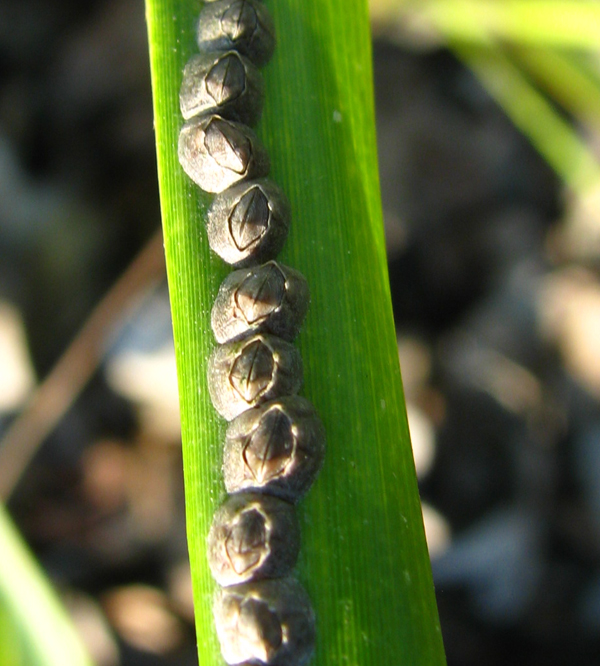
\includegraphics{MEImages/Cfrag.jpg}
\caption{\textbf{Fig.2.6 - A row of \emph{C. fragilis} settled on a stem
of the cordgrass \emph{Spartina alterniflora}. Photo by Y. Zhang,
GCE-LTER.}}
\end{figure}

\emph{Resources cited in this section} Brown, A. et al (2019).

Hamady M, Walker JJ, Harris JK, Gold NJ, Knight R (2008)
Error-correcting barcoded primers for pyrosequencing hundreds of samples
in multiplex. Nature Methods 5: 235--237. 10.1038/nmeth.1184

Katz et al (2009)

\hypertarget{BoxB}{%
\subsection{Box B. An aside to explain these data better and how we
obtain them.}\label{BoxB}}

This would be organized by electrophoresis (mobility, size and charge
and cost) versus sequencing (method, informatics, cost). It will be
brief and use online OA resources to clarify. We will note that later it
will make sense that the information we can glean from sequencing, even
models of thinking about rate and type of mutation, are useful even for
electrophoretic markers and vice-versa.

In order to make any inference such as typical in molecular ecology, you
have to have information. You have to have \emph{variable} information,
in fact. So, the history of this field is in finding ways to recognize
that there is so much diversity in every single sample of life, and do
it efficiently with available technology. As my colleague Jim Hamrick
puts it, it is ``high-tech natural history'' so we often don't have a
lot of funding but we still have big questions!

The trick has been two-fold in our field. At first, we were
technology-limited; it was difficult to obtain information on variable
markers until the advent of protein electrophoresis in the 1960s, but
those offer only a limited view into mutational diversity (and
\emph{may} be frequent targets of selection, see Skibinski \& Ward 2004,
Marden XXXX). Our second problem has often been just as significant,
which is that improvements in technology are often expensive and lets
face it: we are asking questions that don't merit multi-million dollar
NIH grants, in general (though the same methods of course have been
appropriate for asking questions about \textbf{COVID-19}, see Trevor
Bedford and others).

What this means is that the questions you want to ask are often
influenced by how creatively you can use the available funding to do so.
Though in 2020 it is becoming more common to see studies that involve
whole-genome resequencing data - thus, there is a complete view of the
genome, though some may want additional samples, or would still wish for
methylation data, and so on - this is only possible when a
well-scaffolded, complete genome is available. For many of us, that is
simply not true and will not be true for quite some time (or until you
get the \$15-20,000 necessary to buy the data to do it yourself, but
this can easily take a couple of years; Ruiz-Ramos et al 2020).

To save money, there are methods that focus on \emph{anonymous} regions
of the genome, those that focus on \emph{targeted} regions of the
genome, and there are distinctions in how the \emph{targeted} data are
obtained that tend to vary categorically with the number of regions
being evaluated. The ``anonymous'' methods include what is currently
known as genotype-by-sequencing (GBS, and the many flavors of ``RAD''
protocols that are collected to do this) and other methods that involve
shearing the genome into fragments using microbe-derived restriction
enzymes that recognize certain ``words'' in the genome and cleave the
DNA in predictable ways. The extremely common enzyme \emph{Eco}RI comes
from the bacterium \emph{Eschericia coli} and whenever it encounters a
region in double-stranded DNA that has a \textbf{GAATTC} motif, it cuts
the DNA in a way that leaves the **AATT* as a single-stranded
overhanging bit of DNA, for example. What is nice is not only that the
genome has been cut, but an easy way to bind adapter sequences is left
behind for PCR-based methods.

The \emph{targeted} data rely on prior knowledge about a gene region and
its utility for your purposes. For example, probably the most frequently
analyzed single gene region in metazoans is the mitochondrial cytochrome
oxidase I gene region, for the simple fact that Folmer et al.~(1994)
published primers that tend to be able to isolate and amplify that gene
region reliably in metazoans. We have subsequently figured out ways in
which this gene region is particularly useful for molecular ecology, as
well as particular drawbacks it has (Wares 2010) in terms of reliably
transmitting information about mutational events. As scientists have
wanted larger numbers of targeted fragments, the costs of PCR and
sequencing either scale up linearly with the number of targets when
doing traditional PCR and Sanger sequencing (roughly \$1-4 in cost per
\textasciitilde1kb sequence per individual), or larger outlay of cash
for enrichment protocols that allow next-generation sequencing to
provide sufficient sequencing coverage of all the targeted regions. The
cost of the sequencing is one part of the equation (e.g.~in 2020
approximately 110,000,000,000 nucleotides can be returned from an
Illumina sequencer for a cost of less than 1500 dollars), but how
cleverly the underlying experiment is designed strongly affects the
cost-efficiency of this approach.

\begin{figure}
\centering
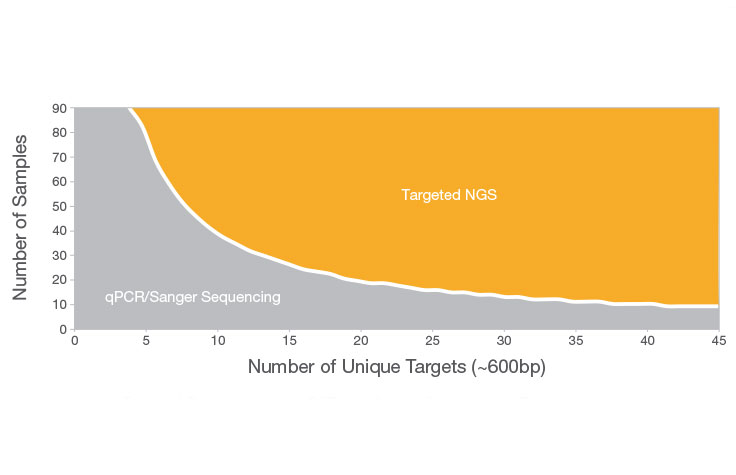
\includegraphics{MEImages/cost-effectiveness-of-targeted-ngs.jpg}
\caption{\textbf{Fig.B1 - From
\url{https://www.illumina.com/science/technology/next-generation-sequencing/ngs-vs-sanger-sequencing.html},
a rough guideline to the benefit of massively parallel ``non-Sanger''
seqeuncing as the number of focal loci increases.}}
\end{figure}

One type of \emph{targeted} loci that can be analyzed efficiently with
electrophoresis, separating fragments by their \emph{size} rather than
their actual sequence, include microsatellite markers or ``simple
sequence repeats'' (SSRs). These loci vary based on short DNA repeats
(e.g.~ATC\textbf{ATC}ATC\textbf{ATC}\ldots or
GT\textbf{GT}GT\textbf{GT}GT\textbf{GT}GT\ldots) that are highly
mutable, and thus these loci tend to harbor higher diversity than other
types of markers but also come along with distinct challenges, both
practical and analytical. The fact that they only require
electrophoresis to genotype an individual would seem to save money, but
the effort to score these loci \emph{and} the overall cost of multiple
PCR reactions and submissions to a genomics center to be run on a
capillary electrophoresis sequencer (often at a cost approaching \$1 per
sample, once costs of cleanup and electrophoresis are included) makes
this of marginal benefit (K. Bobier, pers. comm.), and the cost to
develop these relatively taxon-specific markers (doing enough sequencing
to find the repeat regions whether via enrichment or filtering, primer
design and basic testing - often on the order of thousands of dollars
for a new series) has probably put them into the historical dustbin
except for cases where they already work on your organism.

So, suffice to say there are \emph{so} many ways to collect data
representing genomic variation and you have a few variables to work
with. \emph{How much money is available for this work? How many
individuals should be genotyped, at how many loci, to satisfy your
question?} At this point in the book, you maybe don't know. \emph{How
many individuals do you genotype to figure out whether broods of
barnacle larvae (or seed pods of tropical trees) are fathered by a
single individual, or multiple? How many locations do you need to assay
to understand your overall system - and how many individuals from each
location?} (not to mention the cost and effort of \emph{finding} those
individuals, often a considerable effort itself)

This is the challenge in teaching about the markers. They change
constantly via technology and the availability of resources; the
questions and the statistics used to answer those questions change far
less over time, thus we are going to move forward moving with the
simplest types of data (and simplest types of analysis) first. The
exceptions necessary for dealing with certain types of data - are the
data haploid? Or uniparentally inherited? Are the data dominant or
codominant? In other words, you will also need to understand the
\textbf{natural history} of the markers you are studying, as noted by
famed paleontologist Geerat Vermeij (2003).

A few other notes as we talk about the `natural history' of our markers.
It has been common to talk about loci that are neutral versus those that
are not. Usually, in the context of declaring the data to be neutral
because they are mitochondrial (Avise) or microsatellites, or simply
because they have no known relationship to functional or quantitative
diversity. What we are really saying is that the data have very little
known about this relationship, but that the assumption of neutrality is
often a very very big assumption (Hahn 2008; Rand, Wares 2010, and so
on). The extent to which this type of work is ``genetics'' means that
you have to know how it is inherited (only from maternal? Or is it a
freshwater mussel, and the mitochondrion will reflect paternal diversity
\emph{when in males}), and you have to know how your technique for
capturing it will reflect that diversity - is there potential for null
alleles that do not amplify because of variation in primer sites? Will
you only capture the presence of an allele, and can not distinguish
between homozygotes and heterozygotes? Would you expect the relative
abundance of particular genomic sequences to reliably indicate the
relative abundance of the organisms they come from in an environmental
sample? Why or why not?

So we are going to treat the natural history of loci, and the methods to
obtain the data, as opportunities to consider exceptions to the rule
rather than a basis to build upon. The best data means that you have
sequence data, and a lot of it - and you know what to do with it. Here
we go!

\hypertarget{a-bit-more-biological-reality-and-how-diversity-is-generated}{%
\section{3 A bit more biological reality, and how diversity is
generated}\label{a-bit-more-biological-reality-and-how-diversity-is-generated}}

One last key set of details is going to be important for us knowing how
to ask the right questions using molecular data. So far we have talked
about using molecular assays to find genomic variation in individuals
and samples of individuals. We haven't really talked about where that
variation comes from, and the reason that is important is that almost
all of our questions rely on this variation telling us something about
\emph{rates of change per unit time}.

\hypertarget{how-diversity-is-generated-by-mutation}{%
\subsection{3.1 How diversity is generated by
mutation}\label{how-diversity-is-generated-by-mutation}}

Mutations are errrors. Simple as that. When we teach introductory
biology, there is a single equation for how photosynthesis converts
light and water into glucose and oxygen; but there are any number of
ways in which that metabolic pathway sometimes misses a step or hiccups,
and that becomes more frequent as the environment changes away from the
conditions that a photosynthetic organism is adapted for. So, we
recognize that as ocean temperatures increase, photosynthetic
dinoflagellates living in corals are more likely to produce
tissue-damaging oxygen radicals, and they are ejected by the coral hosts
- causing bleaching. \url{https://www.youtube.com/watch?v=_ZfGIKiSwwQ}

Similarly, mutations happen when DNA replication has an error, as with
`strand slippage' changing the number of repeats in a microsatellite or
adding a G instead of a C as nucleotides are incorporated; or when
ultraviolet light or a chemical toxin damages the DNA and cellular
repair mechanisms don't catch the change.

We should recognize that mutations are happening all the time, though
not always with evolutionary significance. Many cancers are caused by
\emph{somatic} mutations that only affect the diversity in the cell(s)
descended from the initial mutation, for example. However, when
mutations appear in a cell or tissue that has the capacity to reproduce
and make new organisms (``germ line''), those new organisms will carry
the mutation that occurred in the previous generation.

How do we know that mutations happen all the time? First of all, a
rather famous experiment by Luria and Delbrück showed that bacteria
grown from a single cell in a culture medium until there are many
millions of cells have a non-zero probability of a mutation affecting
their tolerance to antibiotics. If the mutations only appeared
\emph{because} of the change in the environment, we would expect a
fairly constant rate of response across replicate experiments; the high
variance in outcomes mathematically showed that mutations were sometimes
happening early in the growth of the culture (so more cells are
resistant when plated on antibiotic medium), sometimes late (very few
cells are resistant), or not at all. That tells us that mutations are
independent from any \emph{response} to the environment; some
environments may promote mutagenicity, but the mutations that arise are
not specific to that environment.

Intriguingly, we can also track mutations happening in long-lived and
clonal organisms. A great example would be aspen trees (\emph{Populus
tremula}), which grow in massive clones with shared root systems.
Distinct clones may be noted during autumn, as leaves turn from green to
brilliant gold, because large patches of trees will all turn at the same
time - but not synchronously with patches next to them. Sequencing
portions of the genome from one edge of a clonal individual and then
from a tree at the opposite edge assumes that the clone is expanding
outwards from its original propagule (seed), and thus many years have
passed since those two sequences came from the same cell. It is typical
to find that these trees on opposite sides of the colony are genomically
distinct (though still clones), and because each tree has its own
reproductive tissues the gametes they produce will carry those distinct
mutations. Similar approaches have been used to look at mutational
diversity in other tree species
(\url{https://doi.org/10.1098/rspb.2019.2364} for \emph{Eucalyptus}, Fig
3.1), and have even been able to use the growth form of trees to
identify the actual rate per amount of tissue growth or per generation!

\begin{figure}

{\centering 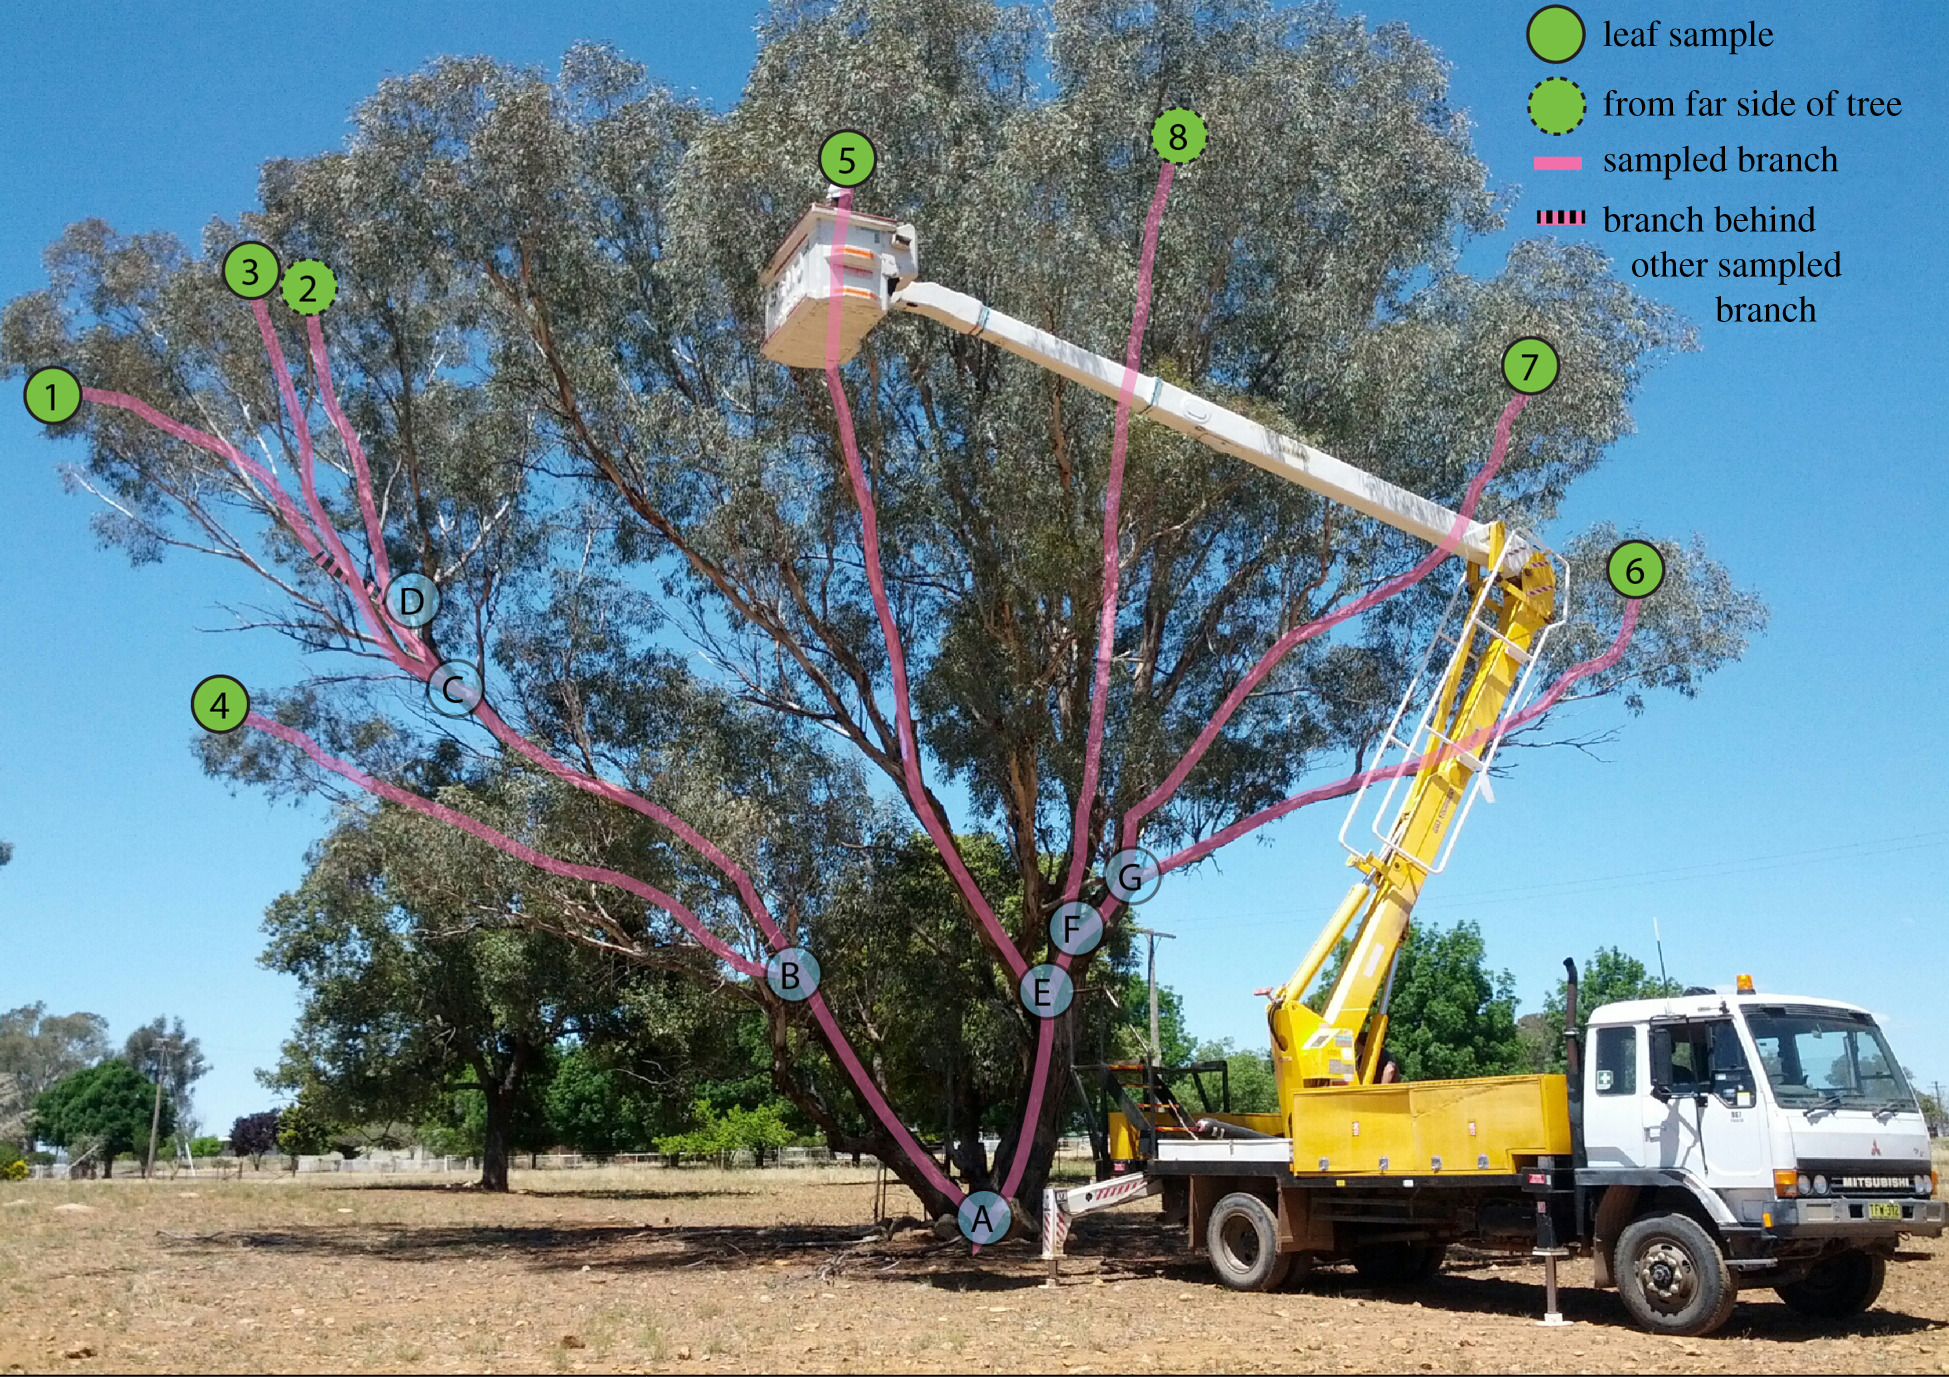
\includegraphics[width=0.9\linewidth]{MEImages/eucalyptus} 

}

\caption{...}\label{fig:unnamed-chunk-2}
\end{figure}

\textbf{Fig.3.1 - From
\url{https://royalsocietypublishing.org/doi/10.1098/rspb.2019.2364},
showing how the `phylogenetic' growth of \emph{Eucalyptus} can be taken
advantage of for studying somatic mutation rates in these trees and
comparing with simpler `model' organisms like \emph{Arabidopsis}.}

A fascinating recent paper by Olsen, Levitan, and others
(\url{https://www.ncbi.nlm.nih.gov/pubmed/30707605} ) looked at this
same question in corals in the Caribbean. Corals tend to start their
life as either a tiny planula larva, created by the formation of a
zygote from spawned eggs and sperm, or as a small chunk of coral that
has broken off from a nearby colony. As the colony grows from this
point, again mutations may happen in individual polyps (each polyp eats,
photosynthesizes, and can reproduce, but all share a common
gastrovascular connection), and mutational diversity can be found
between polyps on either side of the colony. What was really cool about
this work (Olsen et al 2018, \emph{Biological Bulletin}) was that they
evaluated many coral colonies from 2 species, at different depths and
different sizes. The two species have different growth forms and rates,
so the genetic distance between polyps from the same colony depended on
both size and species identity; even more interesting, the mutation rate
was higher for shallow-water colonies, suggesting increased exposure to
ultraviolet radiation from the sun.

\emph{The data in the Olsen et al paper came from microsatellite loci.
As noted in Box B (Chapter 2), this is a method that depends on
isolating and identifying regions in the genome with simple short repeat
(SSR) sequences and then targeting them using PCR. The products are
scored by their relative migration under electrophoresis, using a size
standard that fluoresces a distinct color from the PCR amplicons so that
the products can be scored to size. Though a particular allele may have
14 repeats of ``AGT'' (14 x 3 = 42), the PCR amplicon will include
flanking regions that extend the fragment length so that there is a
space for primers to match for PCR; thus that same allele may actually
be a PCR amplicon that is (for example) 120 base pairs in length. The
fragment length is generally what is scored, and in the best cases each
allele is scored at length intervals that match the repeat element
length (so for the example locus, we might see other alleles at 117,
123, 126 and so on). Later in this chapter we will see more about how
mutational differences are counted among these fragments, but they offer
a highly variable (good) but imperfect view of genome diversity that
requires special consideration.}

These examples from bacteria, trees, and corals are natural examples of
``mutation accumulation'' (MA) studies, which can easily be done (with
time!) in lab organisms with short generation times, such as
\emph{Arabidopsis}, yeasts, and so on. Often of course in order to do
such work you not only need a short-generation organism that is amenable
to culturing in the lab, but also the resources to sequence large
amounts of the genome since the \emph{location} of the mutations will
also be, for the most part, random. To understand how mutation happens
in the rest of diversity, biologists have looked at well-known
geographic features that separated ancestral populations into two or
more descendant populations, and can ask similar questions about how
many mutations distinguish those populations.

Estimating the mutation rate, \(\mu\) , from these long-term isolated
populations requires that we make one additional assumption. Since we
are only looking at the end-point of many hundreds or thousands of
generations of isolation, many mutations will have arisen - and some
will disappear quickly, some will stay in the population as segregating
diversity, and some will go to `fixation' (the novel mutation is now
present in all members of the population). If we assume that the
mutation has absolutely no good or bad qualities with respect to the
survival or reproduction of individuals (``fitness''), then whether it
increases in frequency each generation or decreases is pure stochastic
luck. It depends on the fact that populations are finite in size, and
that for unpredictable reasons not all individuals will have the same
number of offspring - some zero, some one, some many. Because of this
simple fact of variation in reproduction, the frequency of a mutation
changes randomly each generation as shown in this simulation of
\textbf{genetic drift}:

\begin{Shaded}
\begin{Highlighting}[]
\FunctionTok{library}\NormalTok{(learnPopGen)}
\NormalTok{driftplot}\OtherTok{\textless{}{-}}\FunctionTok{drift.selection}\NormalTok{(}\AttributeTok{p0=}\FloatTok{0.2}\NormalTok{,}\AttributeTok{Ne=}\DecValTok{500}\NormalTok{,}\AttributeTok{w=}\FunctionTok{c}\NormalTok{(}\DecValTok{1}\NormalTok{,}\DecValTok{1}\NormalTok{,}\DecValTok{1}\NormalTok{),}\AttributeTok{ngen=}\DecValTok{2000}\NormalTok{,}\AttributeTok{nrep=}\DecValTok{10}\NormalTok{)}
\CommentTok{\#this is terrible slow code}
\FunctionTok{library}\NormalTok{(ggplot2)}

\CommentTok{\#shinyAppFile("/shiny\_popgen{-}master/Drift/drift\_app.R",options=list(width="100\%",height=600))}
\CommentTok{\# how do I get it to start off with frequency 0.2, certain generations and so on?}
\CommentTok{\#run it and download the .csv, read back in and plot it!}

\CommentTok{\#pop500\textless{}{-}read.csv("drift{-}simA.csv",header=T)}
\CommentTok{\#ggplot(data = pop500, aes(x=generation, y=freq)) + geom\_line(aes(colour=sim))}
\end{Highlighting}
\end{Shaded}

The plot shown is based on simulating drift, as we have done before in
this class. In this case, the starting frequency was low (0.2) -- but
not as low as a new mutation -- and the population size \emph{N} is 500.
So that we refresh in our minds how this works, there is also a Shiny
app that lets you control these parameters (nb unless otherwise noted,
the Shiny popgen apps are by Silas Tittes
\url{https://github.com/silastittes/shiny_popgen}).

\textbf{FOR OUR JUNE 1 MEETING WE WILL NOT YET HAVE ACCESS TO THIS
EXERCISE}

\begin{Shaded}
\begin{Highlighting}[]
\FunctionTok{library}\NormalTok{(ggplot2)}

\CommentTok{\#shinyAppFile("shiny\_popgen{-}master/Drift/drift\_app.R",options=list(width="100\%",height=700))}
\end{Highlighting}
\end{Shaded}

Your task with this simulator is to learn about a key understanding
about random genetic drift. Remember, at this point in time all
diversity we have talked about has no known effect on \textbf{fitness}.
You can see from the app above that you can change population size
(\emph{N}), the initial allele frequency, how long (generations) to run
the simulation; *as well as ``bottleneck time'' and ``bottleneck pop.
size''. Don't worry about these last two, but be sure to set
``bottleneck time'' to be greater or equal to ``generations''.

Now, varying \emph{N}, starting allele frequency, generations, and
number of replicates - I'd like for you to set up some simple
observational experiments to \emph{quantify} the probability that the
allele we are tracking (it is at the frequency you set; the other allele
is, of course, at (1-\emph{freq}) in frequency) goes to fixation
(frequency 100\%). I suggest starting with small population sizes, but
then see if it changes as \emph{N} increases.

Second, now that you have run that experiment and described your
approach and results (you will email this to Dr.~Wares), identify the
conditions (including how many loci or observations or replicates are
necessary) that allow an allele starting at frequency 0.01 to go to
fixation. If you increase \emph{N} to 1000, does the likelihood of
fixation change? Or does the time required for fixation change?

Again, email these results to Dr.~Wares \emph{before you read ahead}! If
you are stumped, its OK to email a classmate or email me 😄

OK, now close your eyes, imagine a simulation starting at a frequency
\emph{f} for 2 alleles (that is, one allele at frequency \emph{f}, the
other at frequency (1-\emph{f})). This is an ancestral population. If
that population is, by whatever environmental mechanism, separated into
two distinct populations, how often do you think the two locations being
sampled will have a different allele present in 100\% of individuals?

As you can now recognize, given enough time relative to \emph{N}, there
will be plenty of instances in which a polymorphism goes to fixation in
one location/replicate, and, relative to the ``other''
location/replicate would be a \textbf{substitution}.This small
simulation is not truly realistic in terms of the starting frequency of
a new mutation of course. If there are \emph{N} individuals in a
population, then a brand new mutation would appear at a frequency of
1/\emph{N} (or really 1/2\emph{N} for a diploid locus); but there would
also be many more such opportunities across a whole genome, across many
generations. Kimura's ``neutral theory'' predicts that the probability
of a mutation going to fixation is equal to its frequency when observed,
so with the simulation above in the figure - given enough time - we
would expect 20\% of the simulations to go to fixation and become a
substitution. With a new mutation, that would be a much lower
probability of 1/\emph{N}. However, in each generation you have an
opportunity for mutations to happen on all chromosomes in the
population, in other words \emph{N} times the mutation rate \(\mu\).
Long story short: \textbf{if the mutations are neither advantageous nor
disadvantageous} (neutral, not selected for or against), \emph{the rate
of substitutions is equal to the rate of mutations}.

This means that if we go back to our genetic distances from Chapter 2 -
the mean number of mutational differences between sequences from
populations that have been separated for a long period of time
(\emph{t}) can tell us what \(\mu\) is if we have a good idea of what
\emph{t} is. This, too, is the simplest model for how we approach this
problem and later in the semester we can identify ways to increase the
accuracy of this inference.

\hypertarget{examples-where-we-think-we-know-t-for-this-purpose}{%
\subsection{\texorpdfstring{3.1.1 Examples where we think we know
\emph{t} for this
purpose}{3.1.1 Examples where we think we know t for this purpose}}\label{examples-where-we-think-we-know-t-for-this-purpose}}

Abundant geologic evidence and radiometric dating have shown that
volcanic activity formed the narrow land bridge between South America
and Central America where now Panama and parts of other nations are
found. Prior to this happening, there was relatively free exchange of
marine organisms between the Pacific Ocean and the Caribbean Sea. The
geologic dating estimates that the land bridge had closed off this
passageway around 3.5 million years ago (mya), sundering those marine
populations into demographically distinct Pacific and Caribbean
populations. At this point in time, each population was likely
genomically indistinguishable from the other; but in 3.5 million years,
many new mutations have arisen and gone to fixation in each population,
and we assume those mutations and probabilities to be completely
independent from one another.

Mutation is treated as a Poisson-distributed random process, meaning
that we treat mutations as independent events in a genome, that the rate
is very low but constant for a given time step, and we assume that the
rate is low per time step so that only one event happens at a time.
\url{https://towardsdatascience.com/the-poisson-distribution-and-poisson-process-explained-4e2cb17d459}
This probabilistic assumption can be used to consider how many
lightbulbs must be purchased to keep all lights functional on a
University campus - and the likely number needed to be replaced in any
particular building or room. Importantly, even though the events are
stochastic our estimates of the rate \(\mu\) still relate the number of
events to time.

So, we can look at these separate populations and calculate their
overall divergence \(d_{xy}\) based on the proportional difference of
sequences from the two populations, as in Chapter 2 - and because the
mutation rate \(\mu\) has applied in \textbf{BOTH} populations over the
same stretch of time \emph{t}, that genetic distance is equal to
2\(\mu\)\emph{t}, or \(\mu\)=\(d_{xy}\)/2\emph{t}. In this case, a
famous early study by Nancy Knowlton looked at populations of snapping
shrimp in either basin, assuming \emph{t}=3,500,000 and they estimated
\(\mu\) for typical mitochondrial protein coding loci to be around 2-3\%
divergence per million years. This is called ``calibrating the molecular
clock'' and of course is still a very simplistic way of thinking about
how mutations will arise and be retained in very different parts of the
genome, under different evolutionary mechanisms, but it is a common
starting point for these analyses - and tends to fit well when other
organisms are evaluated, as long as the same gene region is evaluated.

Similar approaches have been taken in instances where we have good
geologic data for the temporary submergence of a land bridge such as the
northern portion of Baja California, allowing new movement across that
land bridge; when erosion allows the headwaters of one river to
``capture'' the diversity of another river, effectively moving the fauna
and flora of the second river into the first and isolating the two
populations afterwards (``river piracy'', J. Waters and others); or when
knowledge of climatic change through time allows us to know when
populations of mice that are now only found on the tops of mountains in
the Rockies used to be connected through gene flow in the valleys during
cooler climates.

\hypertarget{how-we-infer-the-number-of-mutations-thinking-of-whole-genomes}{%
\subsection{3.1.1 How we infer the number of mutations, thinking of
whole
genomes}\label{how-we-infer-the-number-of-mutations-thinking-of-whole-genomes}}

\begin{figure}

{\centering 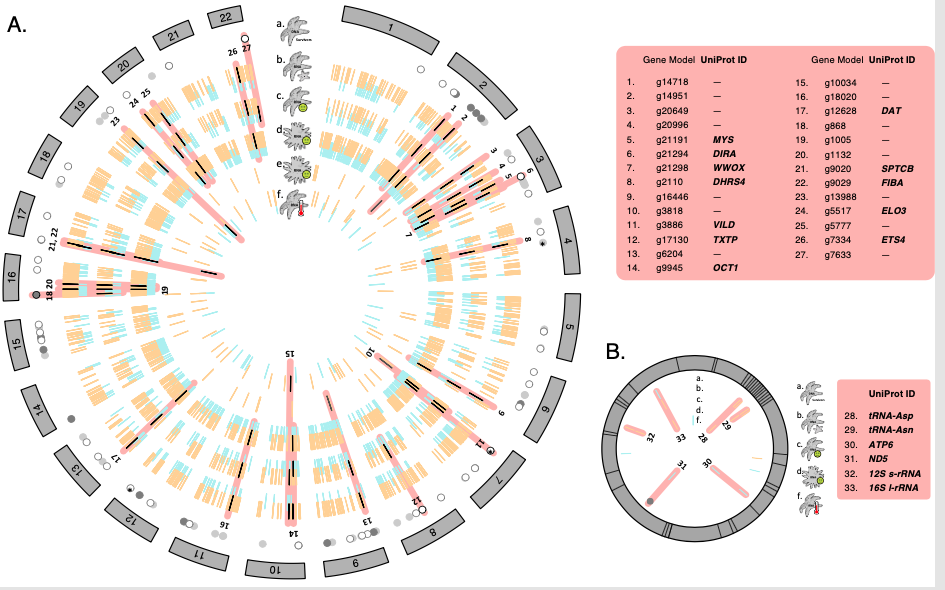
\includegraphics[width=0.9\linewidth]{MEImages/Pisgenome} 

}

\caption{...}\label{fig:unnamed-chunk-3}
\end{figure}

\textbf{Fig.3-2. A `circos' plot of the 22 chromosomes of the
\emph{Pisaster} genome, a number validated by old chromosome squash
data. More internal circles include aligned data of single-nucleotide
polymorphisms from Schiebelhut et al 2018, and differential RNA
expression data from several other studies as summarized in Ruiz-Ramos
et al.~2020.}

A genome is tremendously complex. Figure 4-1 illustrates the complete
genome of the sea star \emph{Pisaster ochraceus}; there are 22
chromosomes (chromosome pairs in a diploid individual), comprising about
400 million DNA nucleotides. Although it is now possible to
`re-sequence' the genome to find polymorphic sites, the complications of
looking for potential gene rearrangements or inversions; dealign with
recombination among sites; and the cost of doing so can be prohibitive
and beyond the needs of a study. A lot of the data used in the field of
molecular ecology are used because they allow a more efficient or
inexpensive analysis that is sufficient for the purposes of the
question. For example, the circles plotted in the first ring inside the
chromosomes represent 100 SNPS (single nucleotide polymorphisms) that
exhibited strong frequency shifts after sea star wasting disease killed
\textasciitilde90\% of all individuals of this species (Schiebelhut et
al 2018 PNAS). The pink radiating bars represent overlap between these
markers and RNA-based expression data that suggest similar responses
across data sets, even across other species influenced by wasting
disease (Ruiz-Ramos et al 2020 Molecular Ecology, where this figure
comes from). How much data, what kind of data, and what sampling
strategy is needed to answer your questions?

Essentially the history of population genetics and molecular ecology
follows the history of technical advances allowing us to see genomic
diversity with greater breadth and resolution. Each technical advance
allows greater consideration of the detail of these data, and so various
models are used essentially to link the identity of any two sequences
(using the term now sensu Hahn 2019 to disambiguate from the two alleles
that each individual carries at a locus, whether identical or not) with
the time since they shared a common ancestor. As with Hardy-Weinberg
equilibrium and the `match' of different ways of evaluating diversity,
when these distinct models generate different estimates of diversity, we
can assume that some evolutionary mechanism is involved, as we will soon
see through examples.

In an ideal world, we know how many mutational events distinguish two
sequences. In this way, we can recognize that mutations may even happen
at the same location in a genome if enough time passes, and so people
studying molecular evolution or phylogenetics of a group of distantly
related organisms will make assumptions about the frequencies of
transitions (a pyrimidine changing to another pyrimidine, or purine to
purine, as with C-\textgreater T or A-\textgreater G mutations), the
frequency of nucleotides in the data, constraints on the molecule such
as codon models, and more in what are called \textbf{finite-sites
models}. Having a tremendous amount of data and complex substitution
models does not guarantee a lack of rancorous debate over the outcome of
such analyses, of course, as with recent discussion of whether
ctenophores (\url{https://en.wikipedia.org/wiki/Ctenophora}) are the
most basal metazoan or not. Those methods are kind of out of the scope
of this class and are often called ``molecular evolution'' or
``phylogenetics/phylogenomics'' or ``molecular systematics'', depending
on the goal of the analysis.

On more recent time scales however, we can make some simplifying
assumptions that work for most of the types of questions we are
interested in as ecologists. A widely-used model is the
\textbf{infinite-sites model}, which assumes that every mutational event
occurs at a new location (site, nucleotide) in the genome and thus the
number of distinctions between any pair of sequences is an indication of
the number of mutations, and that leads us back to inferences of time.
This model applies to cases where we are directly observing at least a
portion of the actual nucleotide data, whether via traditional Sanger
sequencing (a separate reaction for each sequence, individual specimens
are handled distinctly, a total cost of perhaps \$0.005 per nucleotide
per individual per sequence) or high-throughput massively parallel
sequencing with bioinformatic approaches to sort out the data after
sequencing, where many individuals and loci are obtained at once - with
a much higher \emph{minimum} cost to a project, but orders of magnitude
improvement on the cost per nucleotide/individual/locus.

\begin{figure}

{\centering 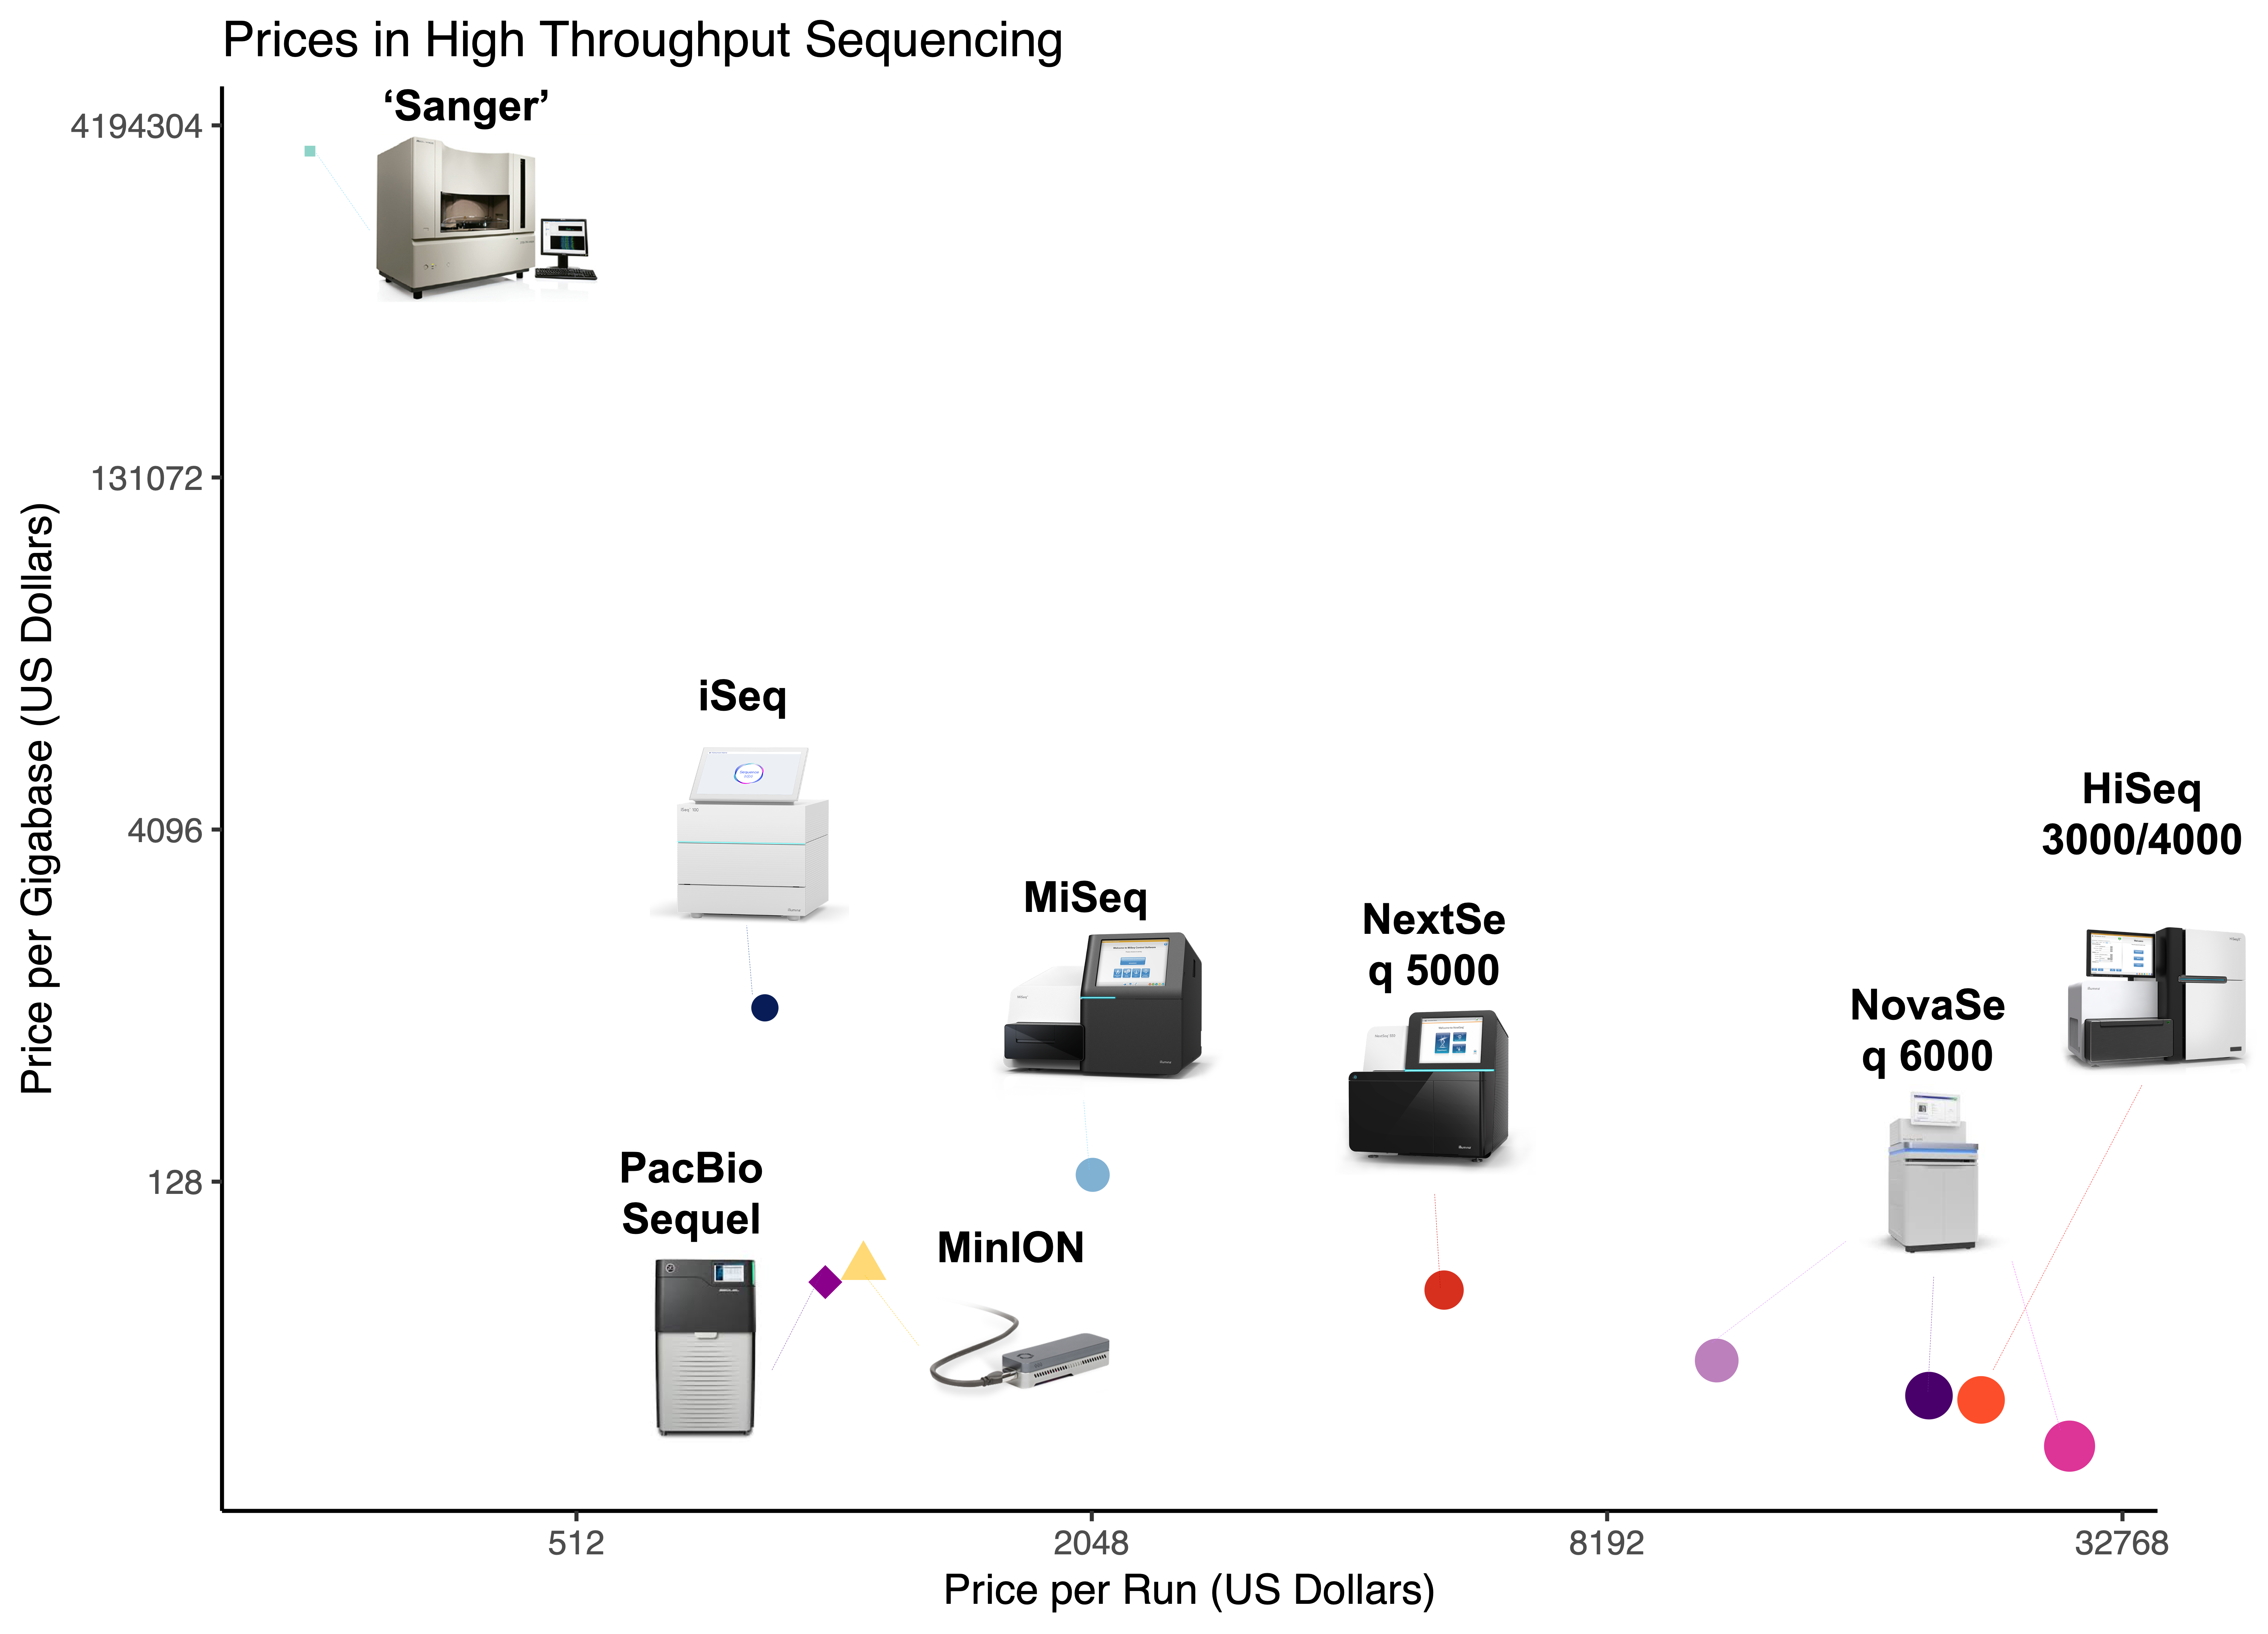
\includegraphics[width=0.9\linewidth]{MEImages/BayonaPicture2} 

}

\caption{...}\label{fig:unnamed-chunk-4}
\end{figure}

\textbf{Fig.3-3. Cost per base pair on different DNA sequencing
platforms; figure by N. Bayona-Vasquez, 2018 - things changing SO fast
though, can now (2020) get 110gigabases of data for \textless\$1500
(e.g.~HiSeqX at novogene.com 😄) but Sanger sequencing costs have not
improved 😦 }

However, until only about 10 years ago, to study multiple loci via
actual DNA sequencing (per locus, per individual) was increasingly
prohibitive in time and money because of the cost of Sanger sequencing
and the effort to get reliable PCR amplicons for highly variable genome
regions (Fig 3-3, see \textbf{Box 1}, e.g.~Wares et al 2009 put a great
deal of effort into having data from 5 loci across roughly 50 individual
chthamalid barnacles). So, an alternative for finding highly polymorphic
loci might be simple-seqeunce repeat (SSR) or ``microsatellite''
markers, where mutations caused by \emph{in vivo} polymerase error lead
to heritable fragment length polymorphisms that are codominant - both
alleles can be known for a locus from a single PCR and electrophoretic
analysis - and could even be multiplexed for reasonable costs per locus
per individual (many studies having 10-20 distinct loci for 10s or 100s
of individual organisms). The drawback to microsatellite markers was
often in their specificity to a particular species, so great effort went
into developing them - and by not evaluating the actual DNA sequence
(and length homoplasy being a common problem), mutational differences
among alleles have to be estimated with something like a
\textbf{stepwise mutation model} (SMM; where fragments of similar length
are assumed to have a more recent common ancestor than with a fragment
of very distinct length) or they are treated as having \emph{unknown}
relationships under an \textbf{infinite alleles model}.

The infinite alleles model (IAM) simply says ``these fragments are
different'' but without knowing whether 1 or 2 or 10 mutational events
happened since they descended from a common ancestral fragment of DNA.
In other words you either have, or are using, far less information in
this case (but it is also a simple model, and not likely to be misled by
big deviations in your assumptions). This model works for protein
electrophoretic variants (allozymes) and some types of dominant markers
as well, and can be used to simplify assessment of sequence variation as
well. For example, in Figure 2.2, 6 sequences are shown and there are 4
distinct alleles represented by that diversity. Without counting the
number of nucleotide differences, we can still represent the number of
distinct alleles under this model; each polymorphic site represents a
mutation that has happened in the history of the sample.

So looking back in time, older data \emph{required} simpler models wtih
less resolution, but those simpler models can still be used to assess
the diversity among a collection of DNA sequence data. As noted above,
the mutational diversity in a sample depends on two things: the mutation
rate, and the number of individuals reproducing. So, we talk about a
population mutation rate \(\theta\) that is the product of these two.
For example, one estimator of \(\theta\) operates under the IAM;
Watterson's \(\theta\), hereafter (W), is just a count of the number of
polymorphic/segregating sites (K) divided by a factor that accounts for
the sample size (larger samples will recover more diversity, typically).

\begin{enumerate}
\def\labelenumi{(\Alph{enumi})}
\setcounter{enumi}{22}
\tightlist
\item
  = \(\frac{K}{a_n}\)
\end{enumerate}

where \({a_n}\) is the sum of 1/\emph{i} from \emph{i}=1 to \emph{n}-1
in a sample of \emph{n} sequences. (W) is an estimator of the population
mutation rate \(\theta\) and a value is obtained from the observed data.
But in our barcode data (Fig 2.2), we already talked about another way
to estimate diversity among sequences; the average pairwise proportional
distance between all sequences in a sample, used at that time to
characterize the distribution of how different sequences might be, is
equivalent to another estimator of the population mutation rate called
\textbf{nucleotide diversity}, or \(\pi\).

\textbf{remember we are still talking about sequence or marker
variation, and not accounting for how it is combined in
diploid/polyploid individuals}

The fact we are currently reading about sequence data, or estimating
mutations between markers that are \emph{proxies} of sequence data (the
length of a microsatellite fragment approximates the knowledge of the
actual sequence, for example), means right now we are not actually
talking about allele frequencies in the same way as in the drift
simulation above. We'll get to that - it turns out that there are
reasons why diploid genomes are more complicated, even though you were
all taught Hardy-Weinberg in high school probably!

The cool thing about (W) and \(\pi\) is simply that they are two related
but distinct ways to estimate how mutational diversity should be
distributed in a population if we assume a single, \textbf{randomly
mating} population with no \textbf{immigration} from other populations,
no \textbf{selection} acting on the diversity, and the
\textbf{mutations} happened before we sampled the diversity. You will
see by Chapter 4 that these are pretty interesting constraints for when
those two estimators should generate the same estimate of \(\theta\).

First, lets revisit what population size \emph{N} does. Because not
every single individual has the same number of offspring - think about
the many acorns an oak tree drops, yet on average \emph{all oak trees}
only replace themselves at best; some will live a lifetime with no
offspring that succeed, others will have many, the average is one in a
stable population. The same could be said for the very few Devils Hole
pupfish; they have a small population size that is absolutely
constrained by the extent of their environment and food resources. If we
start with an assumption of allele frequency - 2 alleles at equal
frequency - how quickly does that allele frequency change?

\begin{Shaded}
\begin{Highlighting}[]
\CommentTok{\#library(learnPopGen)}
\CommentTok{\#oh god I don\textquotesingle{}t see the cache file this takes a LONG time because of first sim; get the cache working}
\CommentTok{\#oakdrift\textless{}{-}drift.selection(p0=0.5,Ne=5000,w=c(1,1,1),ngen=400,nrep=5) \#for now not compiling}
\CommentTok{\#devildrift\textless{}{-}drift.selection(p0=0.5,Ne=100,w=c(1,1,1),ngen=400,nrep=5)}

\CommentTok{\#shinyAppFile("/shiny\_popgen{-}master/Drift/drift\_app.R",options=list(width="100\%",height=600))}
\CommentTok{\# set this for specific params, read back in and plot for them}

\NormalTok{popoak}\OtherTok{\textless{}{-}}\FunctionTok{read.csv}\NormalTok{(}\StringTok{"drift{-}simOak.csv"}\NormalTok{,}\AttributeTok{header=}\NormalTok{T)}
\CommentTok{\#names(popoak)\textless{}{-}c(\textquotesingle{}V1\textquotesingle{})}
\FunctionTok{ggplot}\NormalTok{(}\AttributeTok{data =}\NormalTok{ popoak, }\FunctionTok{aes}\NormalTok{(}\AttributeTok{x=}\NormalTok{generation, }\AttributeTok{y=}\NormalTok{freq)) }\SpecialCharTok{+} \FunctionTok{geom\_line}\NormalTok{(}\FunctionTok{aes}\NormalTok{(}\AttributeTok{group=}\NormalTok{sim,}\AttributeTok{col=}\NormalTok{sim)) }\SpecialCharTok{+} \FunctionTok{ylim}\NormalTok{(}\DecValTok{0}\NormalTok{,}\DecValTok{1}\NormalTok{) }

\CommentTok{\#ggplot(data = popoak, aes(x=generation, y=freq)) + geom\_path(aes(colour=sim) + scale\_y\_continuous(limits=c(0,1),breaks=seq(0,1,0.2)))}

\CommentTok{\#ggplot(data = popoak, aes(x=generation, y=freq)) + geom\_path(aes(colour=sim) + ylim(c(0,1)))}

\CommentTok{\#popoak2\textless{}{-}read.csv("drift{-}simOak2.csv",header=T)}
\CommentTok{\#ggplot(data = popoak2, aes(x=generation, y=freq)) + geom\_line(aes(colour=sim))}

\NormalTok{popdev}\OtherTok{\textless{}{-}}\FunctionTok{read.csv}\NormalTok{(}\StringTok{"drift{-}simDev.csv"}\NormalTok{,}\AttributeTok{header=}\NormalTok{T)}
\FunctionTok{ggplot}\NormalTok{(}\AttributeTok{data =}\NormalTok{ popdev, }\FunctionTok{aes}\NormalTok{(}\AttributeTok{x=}\NormalTok{generation, }\AttributeTok{y=}\NormalTok{freq)) }\SpecialCharTok{+} \FunctionTok{geom\_line}\NormalTok{(}\FunctionTok{aes}\NormalTok{(}\AttributeTok{group=}\NormalTok{sim,}\AttributeTok{col=}\NormalTok{sim)) }\SpecialCharTok{+} \FunctionTok{ylim}\NormalTok{(}\DecValTok{0}\NormalTok{,}\DecValTok{1}\NormalTok{)}
\end{Highlighting}
\end{Shaded}

You'll note a very different amount of change in the oak tree (top)
versus the pupfish (bottom). The point is, the top one has a very large
(effective) population size, the bottom one has a very small one. How we
get to the (effective) part comes later. But do you see the clear
distinction? In a large population, random change happens slowly and
doesn't lose diversity quickly; in a small population, change happens
fast and diversity is lost. We will eventually be able to use this
relationship to look at turnover in allele frequency between distinct
temporal samples from a population and try to estimate what the
(effective) population size actually is; the parentheses are there
because this is hard for all sorts of reasons, but I hope you can
already see it is of ecological interest. One thing you will come across
later is that the because the rate of fixation is faster in small
populations, we can see that the overall rate that heterozygosity is
lost at a locus is \textasciitilde1/\emph{N} per generation, which is
why small inbred populations are of management concern.

So, in finite populations, you will see changes in allele frequency from
generation to generation, and likely it will not - on its own - create
more change than you'd expect from your modest sampling effort of
genotypes to be able to predict allele frequencies. Again, this will
come into play as we try to work backwards from allele frequency shifts
to (effective) population size.

Anyway, that is what happens as time moves forward from a set of
\emph{assumptions} (the allele frequency, the effective population
size). Typically, what we want to do is take observed data and ask
\emph{how they came to be that way} - though predicting the future is
ultimately our goal (Bay et al 2018), we have to first figure out what
we can learn from our reconstruction of the past.

Kingman (1982) is a definitive starting point for understanding the
equivalent model to drift, but moving back in time from the data we can
currently observe. What are those data? In this case, we are assuming
sequence data from a fragment that is large enough to have multiple
sites of mutation (of different ages, thus leading to interesting
patterns) and it is \emph{at least mostly} not recombining within the
history of the sample, which is why there are useful patterns in the
data. We can deal, and will deal, with recombination as well. This is
the problem with models, all of them are wrong because there are always
more complexities in a natural system - but some are useful (quote).

This ``coalescent'' model works with a similar but more explicit
assumption of how each generation is related to the previous. What is
known as the \textbf{Wright-Fisher} model applies to discrete
generations; things can be dealt with, but are somewhat more complex,
with overlapping generations (Charlesworth; Turner et al 2002; Hahn
2019). It is pretty much drift in reverse: if effective population size
is small, it doesnt' take long for the diversity to \emph{coalesce}, to
be descended from a single common ancestral allele or lineage.

So, lets talk about the Wright-Fisher model. This means that you have a
population size \emph{N} and in the previous generation each of those
\emph{N} individuals were descended from \emph{randomly} chosen
ancestors of population size \emph{N}. The ``random'' means that with
probability 1/\emph{N}, 2 individuals have a common ancestor for each
generation back in time (and a probability 1-that, that any 2 do not).
There are fewer good R simulations for this process but this one I like:

\begin{figure}

{\centering 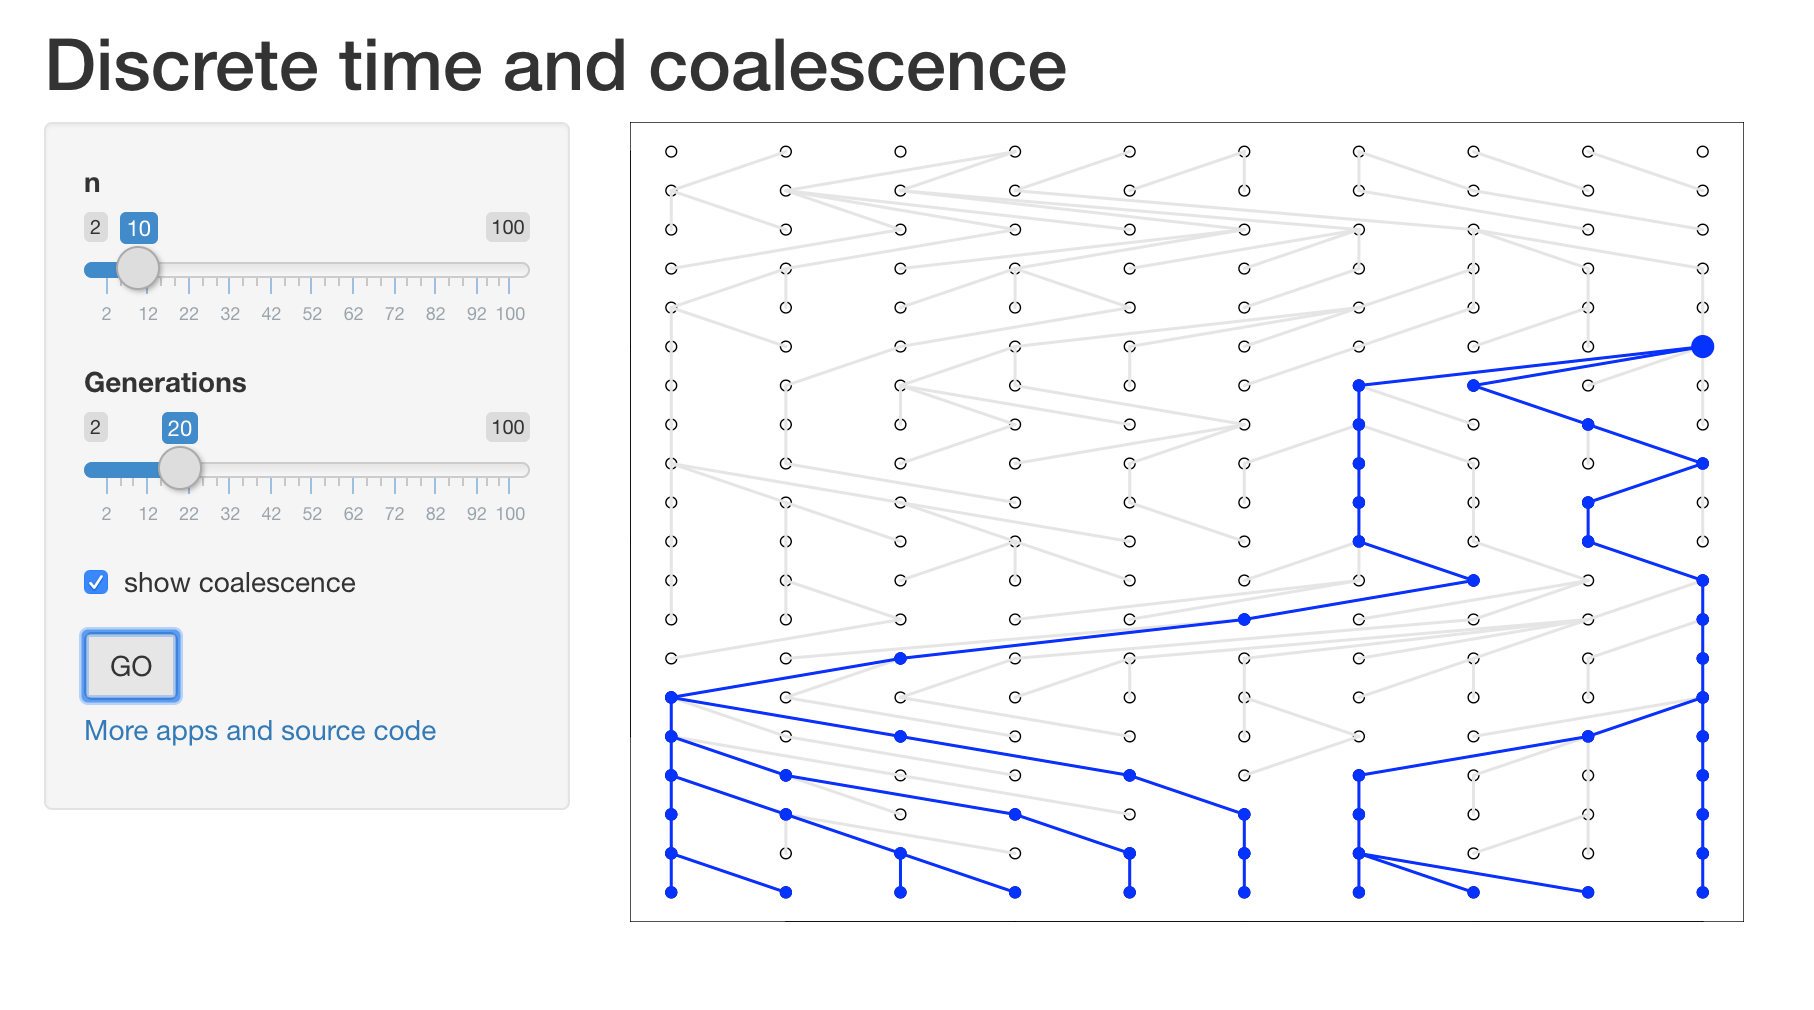
\includegraphics[width=0.9\linewidth]{MEImages/coal1} 

}

\caption{...}\label{fig:unnamed-chunk-5}
\end{figure}

\textbf{Fig.3-x. Coalescent simulator; the SHiny app is below. }

\begin{Shaded}
\begin{Highlighting}[]
\CommentTok{\#shinyAppFile("shiny\_popgen{-}master/Coalescence/discrete\_time\_app.R",options=list(width="100\%",height=600))}
\end{Highlighting}
\end{Shaded}

The top panel is a static image of the Shiny simulation built in below
it. If you set n=10 and generations =20, you can run this simulation
several times and will see very different outcomes. This is a
dramatically oversimplified version of looking at how coalescent theory
works, because in this case the sample size \emph{n} is identical to the
population size \emph{N}, so there are many rapid coalescent events -
but of course as you increase \emph{n} to its maximum (in this
visualization) of 100, you cannot see the events as clearly. It is true
that in very small populations (for example the Florida panthers in the
late 1980s) all individuals sampled will have very recent common
ancestors (both the biological and casual use of term ``inbreeding'').
But the dynamics of coalescent theory have broad implications for
studying genomic diversity in populations of any magnitude.

\begin{Shaded}
\begin{Highlighting}[]
\CommentTok{\#install.packages("coalesceR", repos="http://R{-}Forge.R{-}project.org") did not work right, try again}
\CommentTok{\#library(coalesceR)}
\CommentTok{\#coalescent.plot(n=10,ngen=20)}
\CommentTok{\#get package names}
\CommentTok{\#pckgs \textless{}{-} c("tidyverse", "shiny", "wesanderson")}

\CommentTok{\#determine if packages are installed already}
\CommentTok{\#miss \textless{}{-} pckgs[!pckgs \%in\% installed.packages()]}

\CommentTok{\#install missing packages}
\CommentTok{\#if(length(miss)) install.packages(miss, dependencies = TRUE)}
\CommentTok{\# going to try shiny\_popgen but not sure how to include in Rmd yet...}

\CommentTok{\#shinyAppFile("shiny\_popgen{-}master/Coalescence/continuous\_coalescence\_app.R",options=list(width="100\%",height=600))}
\end{Highlighting}
\end{Shaded}

The Shiny app for coalescent simulation in the above panel is more
technically useful, because you can set the number of sequences sampled
\emph{n} as well as \(\theta\), which you will remember is the product
of the population size \emph{N} and \(\mu\) (and a scalar related to the
number of gene copies). You see that because \emph{N} is much larger
than \emph{n}, the \emph{coalescence} of two sequences happens a much
longer time in the past (and time itself is measured relative to
\(\theta\), so it is not absolute in units of generations or years).
Again, set up the parameters so that you can see that a large number of
highly variable genealogies are consistent with this process, and
mutations are randomly (Poisson distributed by time) placed on the tree.
Together, these generate the patterns of mutational polynmorphism that
we expect when we use (W) and \(\pi\) to estimate \(\theta\). Where this
will get far more interesting, again, is when the basic assumptions of
that single population model are incorrect (Chapter 4).

\hypertarget{how-diversity-is-generated-by-recombination-and-sexual-reproduction}{%
\subsection{3.2 How diversity is generated by recombination and sexual
reproduction}\label{how-diversity-is-generated-by-recombination-and-sexual-reproduction}}

So why have we been working our way through short fragments of haploid
DNA, and talking about quadrats, and now we are talking about whole
genomes? Why isn't a single sample from the genome enough -- isn't that
distinct from sampling the plant diversity of campus or the zooplankton
from a single 1 liter jar taken from a wetland at Savannah River Site?

\begin{figure}

{\centering 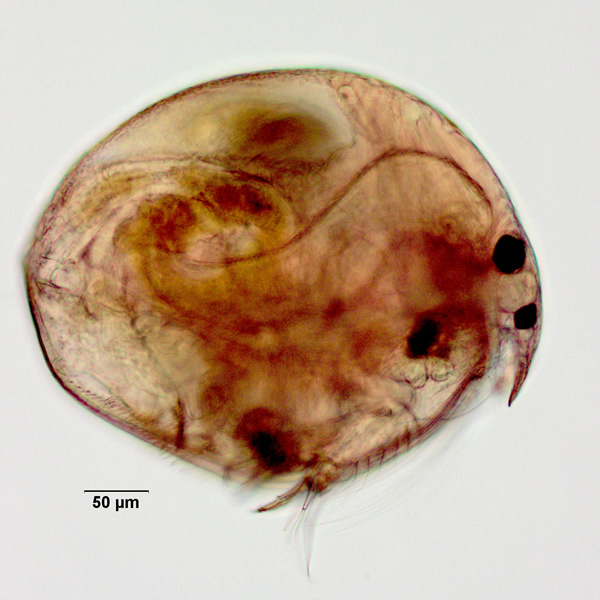
\includegraphics[width=0.5\linewidth]{MEImages/chydorus} 

}

\caption{...}\label{fig:unnamed-chunk-6}
\end{figure}

\textbf{Fig.3-4. A tiny ``microcrustacean'' zooplankton \emph{Chydorus
sphaericus} that is found in freshwater wetlands in the Americas, photo
from
\url{http://cfb.unh.edu/cfbkey/html/Organisms/CCladocera/FChydoridae/GChydorus/Chydorus_sphaericus/chydorussphaericus.html}
}

\textbf{Recombination} is the key here. This is when, during sexual
production of gametes and formation of a zygote, portions of the two
homologous (parental) chromosomes are swapped so that variation from
those two chromosomes can end up next to each other (or linked variation
on one chromosome may get separated). It can be fairly complicated, and
can lead to very interesting patterns, but a basic representation of it
is shown below along with a useful link if you want to learn more.

\begin{figure}

{\centering 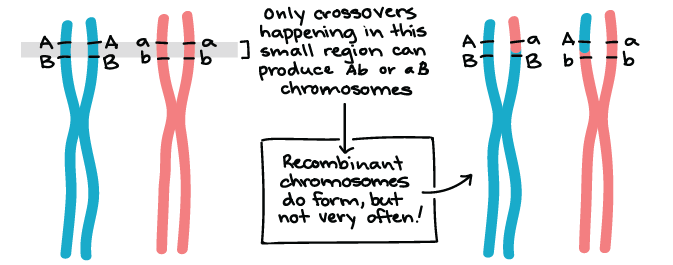
\includegraphics[width=0.9\linewidth]{MEImages/recomb} 

}

\caption{...}\label{fig:unnamed-chunk-7}
\end{figure}

\textbf{Fig.3-5. A simple view of recombination between homologous
chromosomes, not only is this a mechanism that adds overall diversity to
genomes but it means that parts of a chromosome will have a distinct
evolutionary/coalescent/mutational history than other parts of a
chromosome, as shown at right.
\url{https://www.khanacademy.org/science/biology/classical-genetics/chromosomal-basis-of-genetics/a/linkage-mapping}
}

I'm leaving this section short because you didn't sign up for a genetics
class 😄 Recombination complicates things in some ways, but it also helps
us narrow the possible explanations for the data we see. Mathematically,
it is complicated because it changes our bifurcating `trees' expressing
the coalescent history of a sample of whole chromosomes into a graph,
where different portions of the DNA sequence \emph{actually have
different histories}. To the extent we recognize this, however, it means
that distinct loci - whether SNPs obtained by RADseq (\textbf{BOX 1}),
or allozymes (protein electrophoretic alleles), or sequences derived
from targeted PCR fragments - are statistically independent views of the
process of evolution in a population or set of populations, some of them
influenced by effects on fitness or mate choice but most of them acting
as independent observations of the process of genealogical descent and
mutation (drift, coalescence). We can home in on a more accurate
understanding of the history of a population when we have multiple loci.

\hypertarget{the-what-is-a-species-problem}{%
\subsection{3.3 The what-is-a-species
problem}\label{the-what-is-a-species-problem}}

The fact I've brought up recombination means we have to recognize that
most of the diversity we study is diploid (there are mechanisms by which
haploid microbes and mitochondria, etc. also recombine diversity,
however). It's a fascinating transition because having two copies of
each gene can tend to mask the negative consequences of an allele on one
copy, or they can interact in evolutionarily interesting ways (Grosberg
and Strathmann, ``One Cell Two Cell Red Cell Blue Cell'', \emph{TREE}
1998 doi: 10.1016/S0169-5347(97)01313-X.) This is where the fuzzy side
of molecular ecology lies, because sometimes the diversity we are
mapping across space and time will itself interact in interesting ways.

Earlier we mentioned ``inbreeding'', which refers to closely related
alleles (from closely related individuals) and may cause
\emph{inbreeding depression}, when those alleles combine to create a
low-fitness phenotype. Remember, fitness is measured by survival and
fecundity. Later in the book we will talk about conservation and
management approaches based in molecular ecology methods and how they
focus on adding diversity to populations and avoiding mating among
related individuals.

There are plenty of reasons to categorize organisms and groups of
organisms as `distinct' (Chapter 4), and we now see that as more time
\emph{t} passes, portions of the genome become more distinct through
mutation. When we study these divergent alleles using the models we have
discussed, we will see in Chapter 5 just how they show that they cannot
come from a single interbreeding population, and eventually we start
talking about those populations being something entirely different:
species.

When divergent chromosomes interact, the distinct mutations that have
arisen may no longer interact well - they may code for proteins that
don't fit right, or change the timing of flowering or spawning
(\emph{phenology}) such that the combination creates offspring that have
trouble surviving or reproducing. These interactions among very distant
genomes are called \emph{outbreeding depression}, again with a decrease
in fitness. In fact, the greater the divergence between two genomes, or
two populations, at this point it becomes more and more likely that such
interactions will happen (Fig 3-6, Hudson Coyne Turelli; Plough)

\begin{figure}

{\centering 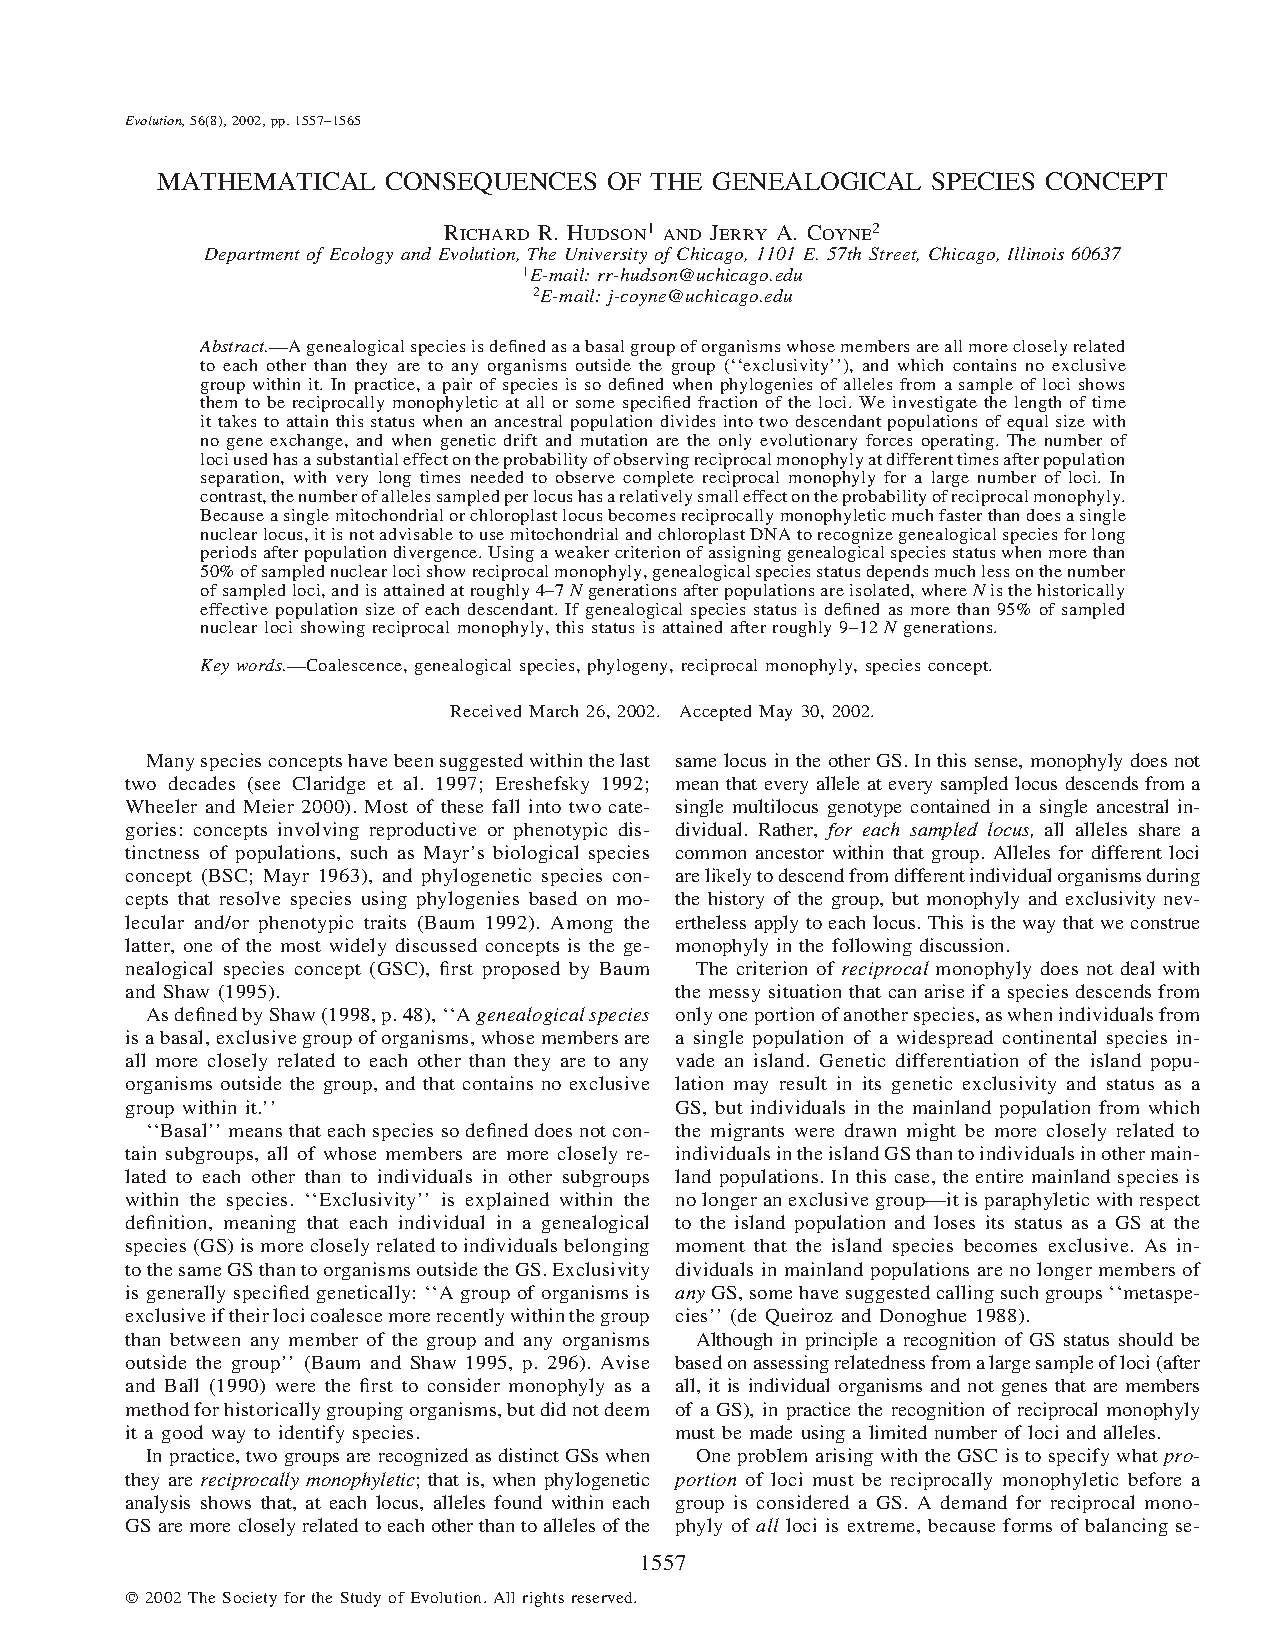
\includegraphics[width=0.9\linewidth]{MEImages/hudsoncoyne02} 

}

\caption{...}\label{fig:unnamed-chunk-8}
\end{figure}

\textbf{Fig.3-6. The variable nature of how long it takes for diversity
in 2 populations to have completely distinct diversity. The more loci
being evaluated, the longer it takes for all of them to reach this
status (in phylogenetic terms known as ``reciprocal monophyly''). A
mitochondrial locus is haploid and maternally inherited, so it has an
effective \emph{N} that is 1/4 that of a nuclear locus}

The figure above shows that with enough time, larger and larger portions
of the genome will be distinct and that adds to the likelihood of
outbreeding depression. The fact that crosses between two such
populations have lower fitness is associated with speciation under what
is known as the ``biological species concept'' (Mayr), but in our field
we are more often diagnosing likely species based on genealogical or
phylogenetic criteria, which are just as valid (de Queiroz 2007). The
trick with drawing any hard and fast rule about ``species'' is that
often there are counterpredictions, as wehn alleles that cause
outbreeding depression (lower survival or reproductioh) vary among
populations of the same apparent species and can even move between
different apparent species when they do successfully hybridize
(Sweigart). Divergence can also be significant simply because of
differences in phenology (flowering, spawning, etc) times among
populations, regardless of the fitness consequences of occasional
crosses, or simple isolation - for many species we just don't know what
happens when they re-encounter one another.

A really fantastic example of this comes from Battey et al 2018, with
one of the most gorgeous figures you will ever see in the field (Fig
3-7). This shows us how genomic diversity varies significantly among
isolated populations of painted buntings on the east coast of North
America versus those in central North America, with distinct migratory
pathways and reproductive isolation based on where they return each year
(R. Chandler: many neotropical migrants return each year within 50m of
where htey were the previous year).

\begin{figure}

{\centering 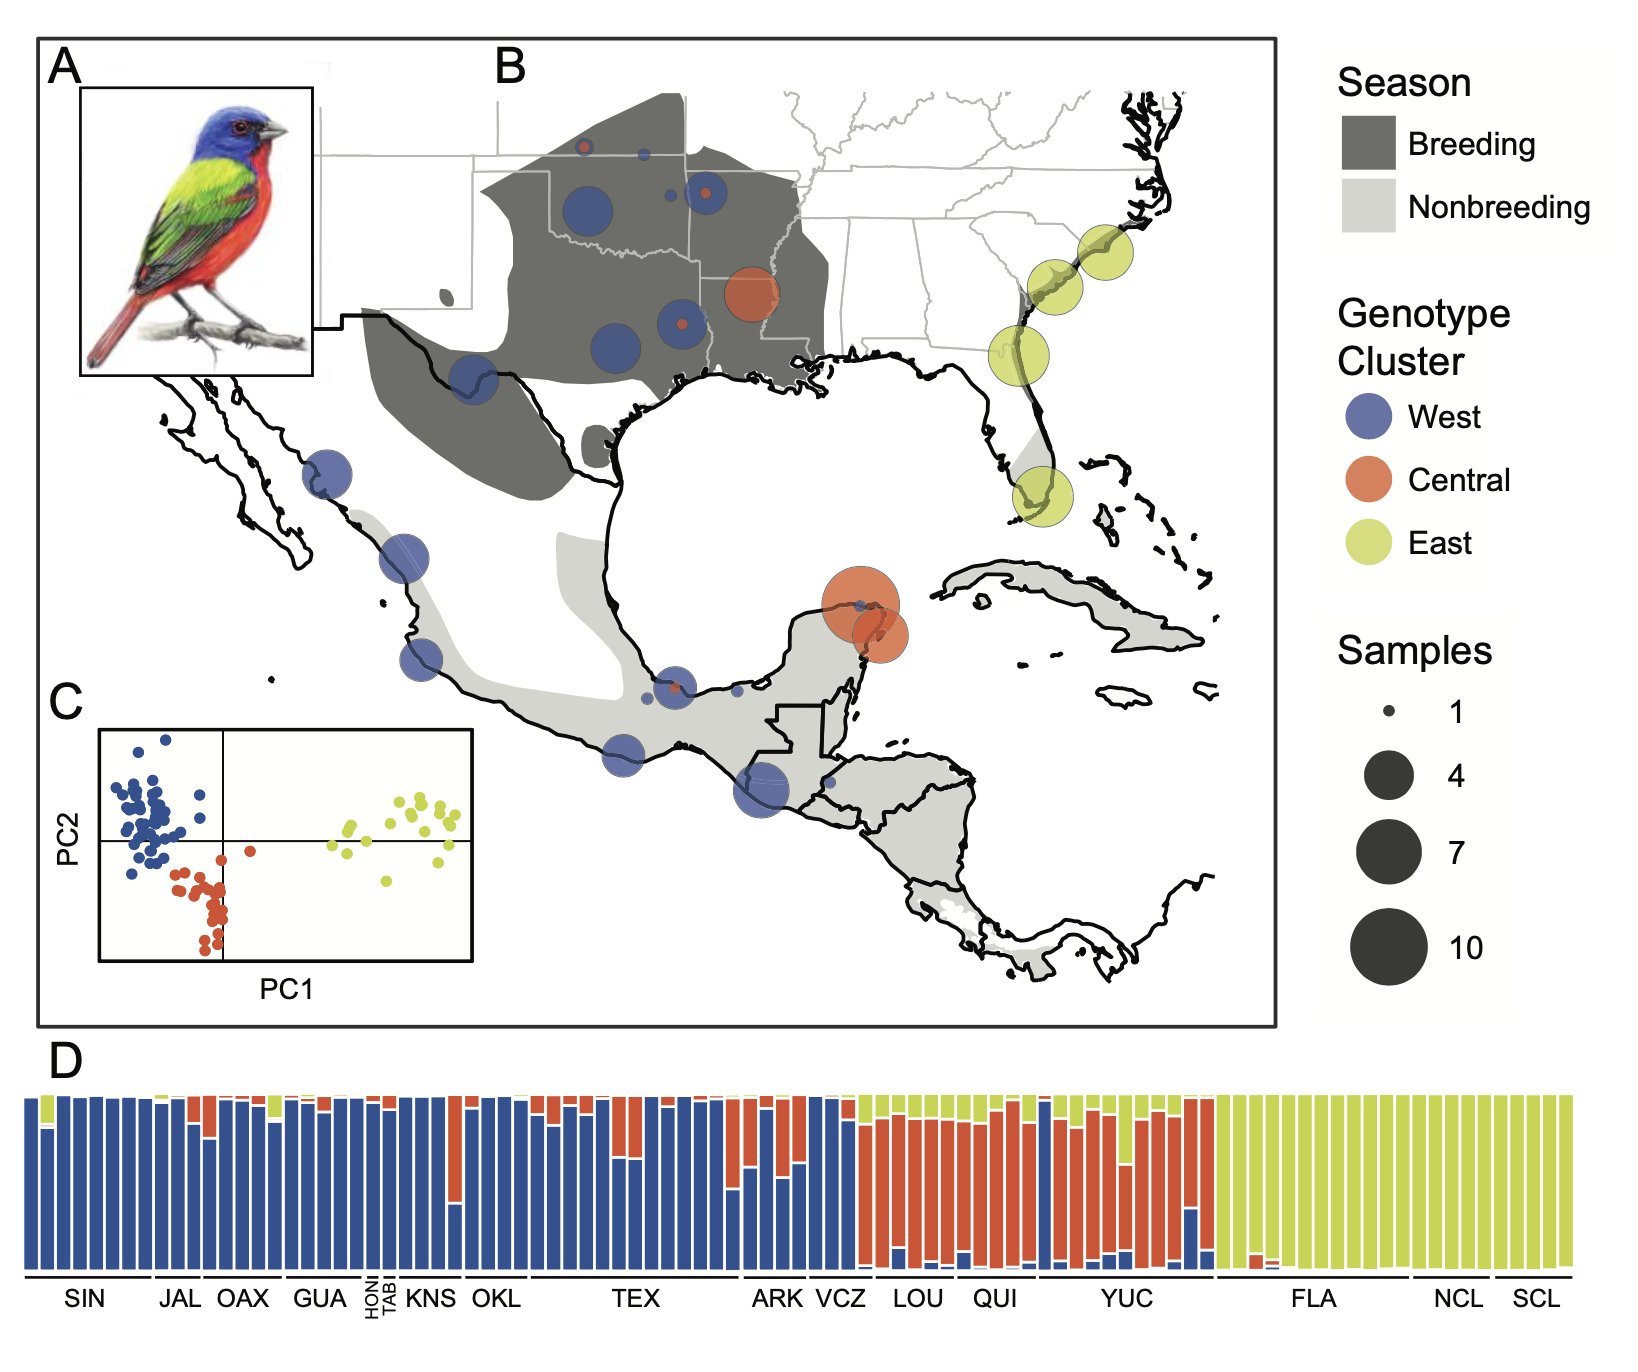
\includegraphics[width=0.9\linewidth]{MEImages/Battey1} 

}

\caption{...}\label{fig:unnamed-chunk-9}
\end{figure}

\textbf{Fig.3-7. Using single nucleotide polymorphisms (over 3600 of
them!) Battey et al 2018 showed that the diversity separates the painted
bunting \emph{Passerina ciris} into 2 very distinct lineages and 3
evolutionarily distinct lineages based on the diversity among the sites
shown. In later chapters we will talka bout the genetic as well as
Euclidean models that let us separate samples of diversity this way.
This is important because it not only highlights where there may be
additional ``species'' within a single Latin binomial, but that there
are ecological and management decisions to be made about how these
distinct lineages migrate and overwinter. }

These data come from ``genotype by sequencing'' approaches, e.g RADseq
or other methods (\textbf{BOX 1}). This means that individual single
nucleotide polymorphisms (SNPs), analytically determined to be unlinked
thanks to recombination, contribute to these patterns. However, as noted
earlier \emph{each individual SNP is only bi-allelic} and so contributes
VERY little information about how these data fit a demographic or
historical model that could be investigated with coalescent methods. The
panel at the bottom (the bar graph) is actually generated by diploid
genotype models discussed in the next chapter. The data involved are
currently state-of-the-art and are beneficial in being so numerous
(remember the advantage of independent views of evolutionary history
thanks to recombination) but for many tests that we will consider later
do not have sufficient information. The way that we will start to look
at these unlinked SNPs will involve a more sophisticated set of summary
statistics (site frequency spectra, genetic inheritance models, etc.) of
DNA polymorphisms - more on this later (\textbf{Chapter 5}).

This is our big overview of how genomic data are used to explore the
diversity of populations, and as you will soon see - mostly, the
deviations from the \emph{null models} that we assume. The next chapter
will discuss how diversity within and among samples is evaluated and how
using genomic data gives us an opportunity to establish these models so
that we can see how mutational diversity can tell us about isolation
among demes, changes in population size, selection, and nonrandom
mating.

The diversity we are looking at starts to `feed back' into generating
functionally distinct things, in different habitats and environments, as
it interacts with both environment and other alleles in the same
organism - fitness consequences are a significant part of what sets the
distribution and abundance of organisms. We will explore how small
amounts of data are used to \emph{predict} the isolation and status of
distinct samples, but more data and experiments are often needed to
identify outbreeding depression or other evolutionary effects (Hickerson
et al 2006). As in Chapter 2, we are often starting from a question of
whether or not it is \emph{important} to characterize populations or
locations as being distinct enough to merit further consideration.

\textbf{As an aside: it seems like I keep pointing the reader to
information that is yet to come. I'm not sure if that is a weakness in
the organization, or if it is recognizign that sometimes you need to be
shown \emph{why} you will want to know those details, and to set up a
little bit of hunger for more. In the end, this may be the deciding
factor in whether this text is useful for future classes or not, and I
will appreciate your input. Personally, I like repetition and
building-on-ideas; nothing in biology seems to be separate from other
elements.}

Your reading for next week is to help us start to think about why some
populations carry more mutational diversity than others - and it is
often not described well by how many individuals there are. The
``effective'' population size I've alluded to describes how the
population diversity \emph{behaves} based on life history traits like
male:female mating ratios, variation in reproductive success, and the
history of a population, and becomes an important consideration in
management and conservation as well as understanding the behavior of
mutational diversity in a sample. So for next week read: Luikart et al
(2010) \emph{Conservation Genetics} \textbf{11}:355-373, linked on eLC.
{[}\emph{meh this wasnt' best choice}{]}

\textbf{ASU students: I'm not only in the beginning of writing this, but
had been writing it for a semester-long class with other papers to read
etc, so pardon the typoes and odd references that aren't needed for what
we are doing at the moment!}

\end{document}
